\documentclass{report}
\usepackage[english,italian]{babel}
\usepackage[utf8]{inputenc}
\usepackage[T1]{fontenc}
\usepackage{hyperref} % i riferimenti diventano cliccabili
\usepackage{graphicx}
\usepackage[table,xcdraw]{xcolor}
\usepackage{dblfloatfix}
\usepackage{longtable}
\usepackage{pdfpages}
\usepackage{enumitem}
\graphicspath{{images/}}


\title{Data Loss Prevention:\\ Sistema di classificazione in grado di identificare documenti che contengono dati sensibili evitandone la diffusione e la perdita}
\author{Paolo Fagioli}


\begin{document}

    % Frontespizio tesi
    
\includepdf{Frontespizio.pdf}

    
    \vspace*{\fill}
    \noindent\rule{\textwidth}{0.4pt}
    \thispagestyle{empty}
    \textbf{Data Loss Prevention} - Sistema di classificazione in grado di identificare documenti che contengono dati sensibili evitandone la diffusione e la perdita.
    \newline
    \newline
    Tesi di Laurea - Università degli studi di Torino
    \newline
    © 2021 Paolo Fagioli. Tutti i diritti riservati.
    \newline
    \newline
    Questa tesi è stata scritta in \LaTeX.
    \newline
    \newline
    Matricola: 859461
    \newline
    \newline
    Email: paolo.fagioli@edu.unito.it
\pagebreak
    
    % Ringraziamenti
    %\begin{flushright}
    \thispagestyle{empty}
    Ai miei genitori,\\
    il mio punto di riferimento,\\
    che mi hanno sempre\\
    supportato e incoraggiato\\
    nelle mie scelte.\\
\end{flushright}

\begin{flushright}
    Ai miei colleghi di corso e amici,\\
    Le persone con cui ho\\
    condiviso attimi\\
    di felicità e tristezza.\\
\end{flushright}

\begin{flushright}
    A Lavinia,\\
    per avermi sopportato\\
    tutto questo tempo\\
    ed esserci sempre stata\\
    nei momenti difficili.\\
\end{flushright}

\begin{flushright}
    E infine,\\ 
    a me stesso,\\
    per non aver mai mollato\\
    nonostante tutto.
\end{flushright}

\begin{flushright}
    Grazie
\end{flushright}

    %Dichiarazione
    \chapter*{\centering \textsc{Dichiarazione di originalità}}
\thispagestyle{empty}

``Dichiaro di essere responsabile del contenuto dell'elaborato che 
presento al fine del conseguimento del titolo, di non avere plagiato
in tutto o in parte il lavoro prodotto da altri e di aver citato le fonti
originali in modo congruente alle normative vigenti in materia di plagio e 
di diritto d'autore. Sono inoltre consapevole che nel caso la mia dichiarazione
risultasse mendace, potrei incorrere nelle sanzioni previste dalla legge e la 
mia ammissione alla prova finale potrebbe essere negata.''

\begin{flushright}
    - Paolo Fagioli
\end{flushright}

    % Abstract
    \selectlanguage{english}
    \begin{abstract}
        \selectlanguage{italian}

Questo lavoro è frutto della mia esperienza di tirocinio compiuta presso l’azienda \textsc{Certimeter Group}. Il mio stage si è incentrato su tematiche inerenti al mondo della sicurezza informatica, in particolare sulla gestione della prevenzione in materia di perdita dei dati (Data Loss Prevention).

Per Data Loss Prevention s’intendono sistemi e tecniche che permettono di prevenire delle perdite di dati e la loro diffusione. Esistono diversi tipi di sistemi che si focalizzano sulla protezione dei dati in momenti di vita diversi. 
Ho avuto modo di conoscere tecniche per la protezione dei cosiddetti dati a riposo, dei dati in movimento e dei dati in uso. 

Il tirocinio mi ha portato a confrontare i principali prodotti presenti sul mercato per capire quali sono le caratteristiche fondamentali che contraddistinguono una soluzione DLP.

Il mio progetto consiste nell’implementazione di una soluzione DLP per la protezione di uno di questi tipi di dati. Personalmente, ho deciso di implementare un sistema per la protezione dei dati in movimento.

La soluzione DLP implementata permette di monitorare il traffico email, ispezionando il contenuto di ciascuna, in modo da identificare quelle che contengono dati sensibili così da prevenirne la perdita ed evitarne la diffusione.

La scelta di implementare questa funzionalità è dovuta al fatto che le email sono, uno dei metodi di comunicazione più utilizzati e conosciuti da tutti, e in modo particolare, il principale metodo di comunicazione in ambito aziendale.

L’implementazione comporta l’utilizzo di un relay Mail Server, Postfix, configurato in modo tale da ispezionare il contenuto delle email e di compiere delle azioni, quali, il blocco della consegna, o la quarantena, del messaggio, in caso dovesse rilevare la presenza di dati sensibili.

La soluzione implementata ha l’obiettivo di incrementare i livelli di sicurezza in ambito aziendale, per questo motivo andrà ad interfacciarsi con il client di posta elettronica standard utilizzato in azienda, Microsoft Outlook, e il server di posta elettronica aziendale Aruba.




\begin{figure}[b]
    \centering
    
\includegraphics[scale=0.07]{logo_certimeter.png}
\end{figure}
    \end{abstract}

    \selectlanguage{italian}

    % Indice
    \tableofcontents
    %\thispagestyle{empty}

    % Capitoli
    \chapter{Introduzione}

Nel settore aziendale si è rilevato, soprattutto nell’ultimo periodo causa pandemia da COVID-19, un aumento delle minacce e un incremento del pericolo di furto di identità o di informazioni rispettivamente a carico del singolo o delle aziende.

Poiché è necessario contrastare questo tipo di minacce, oltre a prevedere i classici sistemi di protezione perimetrale come i firewall, è assolutamente necessario prevedere sistemi che impediscano alle informazioni di uscire dai sistemi aziendali: i cosiddetti sistemi di Data Loss Prevention (DLP).

Benché i firewall siano le difese perimetrali più conosciute, in grado di filtrare in base a indirizzi ip sorgente e destinazione, porte, e sul tipo di protocollo utilizzato, non sono in grado di identificare eventuali dati sensibili.

Questa tesi si concentra sullo sviluppo e l’implementazione, fino al collaudo e al Go Live di un sistema DLP in grado di identificare dati sensibili, all'interno delle email, così da prevenirne la perdita ed evitarne la diffusione.

\section{Organizzazione}

Il capitolo 1 introdurrà una breve introduzione della tematica della Data Loss Prevention.

Nel capitolo 2 verrà effettuato un confronto tra i principali prodotti presenti sul mercato per capire 
quali sono le caratteristiche fondamentali che contraddistinguono una soluzione DLP.


All’interno del capitolo 3 sarà descritto, in breve, il tipo di soluzione implementata e verrà 
effettuata l’analisi e il disegno del progetto.


Il capitolo 4 presenterà in generale Postfix e come sarà utilizzato per soddisfare i requisiti 
scoperti durante la fase di analisi.


Nel capitolo 5 verrà effettuata l’installazione e configurazione di 
Postfix in modo che si interfacci con il mail client utilizzato in azienda Outlook e che svolga 
la funzione di mail server di inoltro verso il servizio di posta elettronica aziendale di Aruba. 
Per garantire la sicurezza, il traffico viaggerà utilizzando canali di comunicazione sicuri/cifrati.


Il capitolo 6 tratterà lo sviluppo di filtri interni per l’analisi del contenuto e del contesto attraverso 
l’uso di parole chiave e di espressioni regolari.
Sarà anche sviluppato uno script esterno in Python per l’analisi del contenuto degli allegati e successivamente 
verrà integrato in Postfix. Succederà a questo una fase di testing.


Infine un ultimo spazio è dedicato alle conclusioni e ai possibili sviluppi futuri.

    \chapter{DLP e posta elettronica}

In questo capitolo si riportano gli aspetti teorici principali riguardanti la tematica della Data Loss Prevention
e viene descritto il funzionamento della posta elettronica, in modo da comprendere al meglio i capitoli
successivi.

\section{Data Loss Prevention}
Con il termine Data Loss Prevention si fa riferimento a 
tecniche e sistemi in grado di identificare, monitorare 
e proteggere dati riservati con l’obiettivo di individuare 
e prevenire l’uso non autorizzato e la diffusione di informazioni riservate \cite{DLP1}. 

Vi sono diversi tipi di minacce che possono portare ad una perdita di dati.
La perdita di dati, in un'azienda, può avvenire accidentalmente, per negligenza di un 
dipendente. È possibile che a provocare una perdita di dati sia un dipendente malintenzionato,
mosso dall'intenzione di danneggiare l'azienda o di rubare informazioni al suo datore di lavoro.
Vi è anche la possibilità che un hacker, attraverso tecniche di ingegneria sociale, riesca a rubare
le credenziali di un dipendente e ad intrufolarsi all'interno della rete aziendale, ovviamente con 
l'obiettivo di appropriarsi di dati riservati.
Queste sono alcune delle possibili vie che possono causare una perdita di dati. Poiché una perdita di dati
può comportare sanzioni, conseguenze legali, ingenti perdite economiche, fino al compromettere la reputazione del 
marchio e portare al fallimento dell'azienda, è necessaria l'implementazione di soluzioni
DLP\footnote{\textit{DLP}: Data Loss Prevention}.
 

\subsection{Cosa fa una soluzione DLP}
    Una soluzione DLP monitora il traffico dei dati all'interno di un'azienda per accorgersi se
    questi circolano impropriamente. In caso di anomalie, vengono attivate delle azioni di risposta 
    in modo da bloccare il trasferimento dati non autorizzato e prevenire quindi la loro perdita/diffusione \cite{DLP2}.
    


\subsection{Tipi di dati monitorati}
    Nota l'importanza dei dati che le soluzioni DLP si occupano di proteggere,
    ora, è opportuno spiegare cosa s'intende quando si parla di dati riservati e che tipi di dati vengono monitorati 
    da una soluzione DLP. I dati riservati sono dati che hanno maggior valore per un'azienda e che possono comportare 
    delle conseguenze se vengono persi o divulgati.

    In natura esistono due tipi dati: \textit{dati strutturati e non strutturati}.
        \subsubsection{dati strutturati}
            I dati strutturati sono dati che, come dice il nome, hanno una struttura, che presentano un pattern comune, e che 
            quindi possono essere facilmente individuati tramite le espressioni regolari. 
            Sono esempi di dati strutturati numeri delle carte di credito, codici fiscali, eccetera.
            Il 20\% dei dati sono di tipo strutturato. 
    
            \begin{center} 
                \textit{Espressione regolare per carte di credito Visa Mastercard:}
                \verb/^(?:4[0-9]{12}(?:[0-9]{3})?|5[1-5][0-9]{14})$/ 
            \end{center}

        \subsubsection{dati non strutturati}
            I dati non strutturati, a differenza dei precedenti, non presentano un modello ripetibile
            e quindi prevedibile. L'80\% di tutti i dati rientra in questa categoria. Esempi di dati non 
            strutturati sono email, immagini, audio, video, file pdf, eccetera. 
    
    Le espressioni regolari non sono adatte per identificare questo tipo di dati. %(possono essere usate per l'estrazione di informazioni strutturate da dati testuali non strutturati), 
    Per i dati non strutturati si usano tecniche differenti, più sofisticate, alcune delle quali sono introdotte nel paragrafo successivo \cite{DLP3}.

    \subsubsection*{}
    I dati, durante la loro vita, possono trovarsi a riposo, in utilizzo o in transito.
    L'obiettivo della DLP è quello di proteggere i dati nei diversi stati in cui si possono trovare:
    \cite{DLP1}

    \subsubsection{data-at-rest}
        I dati a riposo sono dati al momento inattivi, che sono immagazzinati fisicamente in database,
        o in file (ad esempio in file excel), oppure su dispositivi di storage come HDD o SSD, eccetera.
        Se sono salvati in un computer, questi dati si trovano in memoria secondaria.
        Le modalità di protezione di questi dati sono denominate DARP\footnote{\textit{DARP}: Data At Rest Protection}, 
        di cui fanno parte tecniche come la crittografia dei dati (prima di essere archiviati) oppure come la cifratura
        dell'intero dispositivo di storage, protezione con password, il controllo degli accessi, eccetera.

    \subsubsection{data-in-use}
        A differenza dei dati a riposo, questi sono dati attivi, ovvero dati che stanno venendo
        visualizzati o manipolati da un'applicazione, dati con cui un utente sta interagendo. 
        Questi dati si differenziano dai dati a riposo perché, essendo al momento in utilizzo, 
        si troveranno in qualche registro della CPU, in qualche cache 
        o comunque in memoria principale. Sono più complessi da proteggere perché, dato che l'utente vi sta
        interagendo, si troveranno necessariamente in chiaro. Per la protezione di questi tipi di dati
        vengono usate tecniche che bloccano l'uso delle porte fisiche, il copia e incolla, gli screenshots, l'uso dei fax
        e delle stampanti.

    \subsubsection{data-in-motion}
        Sono dati in transito quei dati che al momento stanno attraversando una rete per raggiungere 
        una destinazione finale. Le misure di protezione dei dati in transito sono fondamentali in quanto
        i dati sono considerati meno sicuri durante il movimento.
        Alcune tecniche di protezione base sono la cifratura dei dati
        e l'utilizzo di connessioni sicure (HTTPS, FTPS, TLS/SSL, SMTPS).

  %      \begin{figure}[htp]
    %         \vspace{0.5cm}
    %        \centering
     %       \fbox{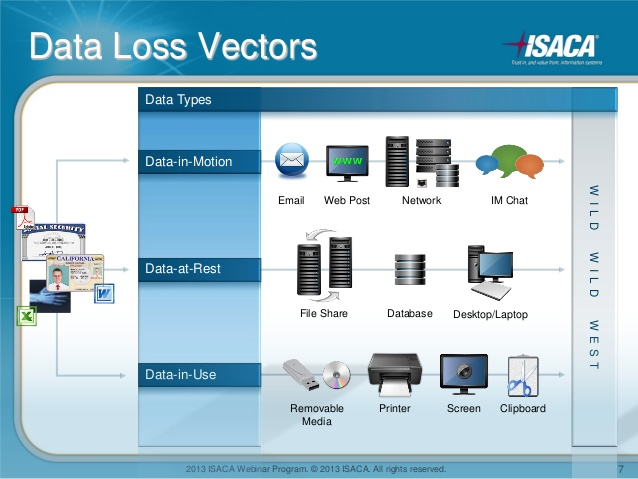
\includegraphics[width=.8\textwidth, height=.6\textheight, keepaspectratio]{data loss vectors.jpeg}}
      %      \caption{Modello ISACA: Data Loss Vectors}\label{ModelloIsaca}
       %   \end{figure}
%\pagebreak
\subsection{Identificazione dei dati}
    Vi sono diversi metodi per l'identificazione di dati riservati, l'utilizzo di una tecnica piuttosto che
    un'altra dipende se il dato è strutturato o meno. Di seguito 
    una breve spiegazione su alcune delle tecniche per identificare dati riservati: \cite{DLP4}
    \subsubsection{Pattern matching}
    Questa tecnica si basa sull'utilizzo delle espressioni regolari che hanno come scopo quello
    di identificare pattern prestabiliti. Come detto in precedenza è la tecnica maggiormente 
    utilizzata per i dati strutturati. 

    \subsubsection{Dictionary lookup}
    La tecnica del dizionario si basa sull'utilizzo di un file di testo che ha come funzione quella
    di un vero e proprio dizionario. All'interno, il file viene riempito di parole chiave. 
    Il dizionario viene utilizzato come database di confronto per identificare dati riservati all'interno 
    di documenti. Questo metodo è particolarmente adatto per dati non strutturati.

    \subsubsection{File fingerprinting}
    Anche questa tecnica è utilizzata per dati non strutturati come file, immagini, eccetera.
    Attraverso questa tecnica si può confrontare l'impronta di un file inviato via mail con 
    le impronte di file riservati precedentemente calcolate, salvate in database.
    Se ad esempio l'impronta del file in transito coincide con una di quelle del database,
    allora il file è un file riservato e si deve bloccare la sua diffusione.

\subsection{Network DLP vs Endpoint DLP}
    Nel mercato sono presenti diversi tipi di prodotti DLP, ognuno dei quali si concentra sulla protezione
    di un diverso tipo di dato. I principali sono i network DLP che si concentrano sulla protezione dei dati
    in transito, e gli endpoint DLP che invece sono incentrati sulla protezione dei dati in uso.
    Non vi è un prodotto migliore dell'altro perché ognuno presenta dei vantaggi e non è esente da difetti.

    \subsubsection{Network DLP}
            È inserito all'interno di una rete. Può comportare un minimo di overhead poiché tutto il traffico
            passa attraverso il dispositivo DLP per essere analizzato.
            Il network DLP monitora i dati che attraversano la rete e applica le politiche che sono in vigore
            in quel momento. Quando ad esempio un utente prova ad inviare un file riservato utilizzando la posta
            elettronica, il  dispositivo nDLP ispeziona il traffico e attraverso criteri predefiniti 
            può bloccare, mettere in quarantena o crittografare la email.
            Uno svantaggio di questo dispositivo è che se il device non si trova all'interno della rete aziendale,
            e non viene utilizzata una corporate VPN, il nDLP non ha visibilità su cosa stia succedendo con quei 
            dati.

    \subsubsection{Endpoint DLP}
            Consiste in un agent che va installato in ogni computer che si vuole monitorare. A differenza del precedente 
            però l'eDLP protegge sempre i dati, anche quando il computer non è all'interno della rete aziendale, ma ad esempio in un 
            aeroporto, utilizzando una rete pubblica. Un endpoint DLP permette di implementare le tecniche di sicurezza
            citate precedentemente per la protezione dei dati in uso. un eDLP può ad esempio proteggere file riservati
            dall'essere copiati su pendrive o HDD esterni.
    
    \subsubsection*{}     
    Essendo prodotti con obiettivi diversi, è consigliato che le aziende utilizzino una soluzione che comprenda entrambi
    in modo da essere protette su più fronti \cite{DLP5}.


\pagebreak
\section{Posta elettronica}
La posta elettronica è uno dei servizi Internet più utilizzati in tutto il mondo \cite{posta}. Attraverso di essa
è possibile scambiare messaggi attraverso la rete in modo facile, veloce e soprattutto gratuito. 
I messaggi scambiati possono consistere in semplice testo (oggetto e corpo), 
oppure includere anche uno o più allegati.

\subsection{Formato dei messaggi di posta elettronica}
Un messaggio di posta elettronica contiene una serie di righe di intestazione (header).
Ogni intestazione è una coppia \textit{chiave: valore}. Alcune parole chiave sono opzionali (Subject:), 
ma altre sono obbligatorie come From: e To:. Una riga vuota separa gli header dal corpo del messaggio.
Di seguito un esempio di messaggio di posta:

\begin{verbatim}
    User-Agent: Microsoft-MacOutlook/16.49.21050901
    Date: Wed, 19 May 2021 12:12:08 +0200
    Subject: Importante
    From: Paolo Fagioli <paolo.fagioli@certimeter.it>
    To: Paolo Fagioli <palfag33@gmail.com>
    Message-ID: <9C8047BB-21D6-4D68-B33E-CCF3B68399DB@certimeter.it>
    Thread-Topic: Importante
    Mime-version: 1.0
    Content-type: text/plain;
        charset="UTF-8"
    Content-transfer-encoding: quoted-printable

    Invio un messaggio di prova.
    Saluti,

    Paolo Fagioli
\end{verbatim}

\subsection{Architettura del sistema di posta elettronica}
La posta elettronica è basata su un'architettura client-server. 
Sia lato mittente che lato ricevente, viene utilizzata un'applicazione, lo user agent, per rispettivamente 
comporre ed inviare, e leggere i messaggi ricevuti. 
Alcuni esempi di user agent sono Microsoft Outlook, utilizzato per lo sviluppo della soluzione DLP, 
e Mozilla Thunderbird.
Un altro componente fondamentale per il funzionamento della posta elettronica è il mail server. 
Un mail server svolge principalmente due funzioni:

\begin{enumerate}
    \item salva il messaggio nella casella di posta dell'utente (è importante sapere che ogni utente ha una casella di posta salvata in un qualche mail server);
    \item inoltra i messaggi di posta verso un altro mail server.
\end{enumerate}

Il protocollo principale utilizzato per lo scambio di messaggi di posta elettronica è SMTP, 
che viene affrontato nel paragrafo successivo.
Attraverso il seguente esempio verrà illustrato il funzionamento della posta elettronica.
Supponiamo che Alice (alice@topolino.it) voglia inviare un messaggio a Bob (bob@paperino.it).

Alice avrà composto il messaggio utilizzando ad esempio Outlook, e lo invierà al proprio mail server 
sfruttando il protocollo SMTP. Una volta ricevuto il messaggio, il mail server di Alice si incaricherà di 
inoltrare quest'ultimo verso il server di posta di Bob (generalmente non sono utilizzati server di posta intermedi, 
ma le connessioni avvengono direttamente tra i server di posta finali). 
Una volta ricevuta l'email, il server di posta di Bob la immagazzinerà nella sua casella di posta. 
Successivamente quando Bob controllerà la sua mail, il messaggio di posta verrà scaricato dallo user agent 
utilizzato da Bob, si ipotizzi Thunderbird, rendendolo disponibile alla sua vista.
La figura \ref{architetturaPosta} riassume i vari componenti che partecipano al trasferimento del messaggio, dal
mittente al destinatario, e i relativi protocolli utilizzati \cite{kurose2008reti}.

\begin{figure}[htp]
    \centering
    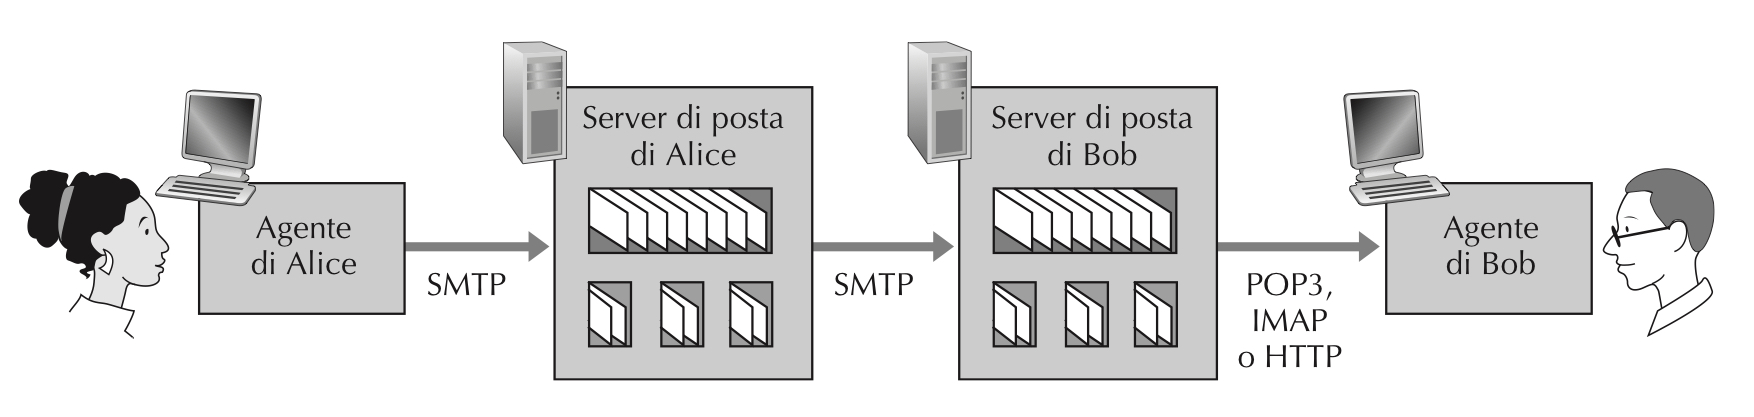
\includegraphics[width=12cm, height=20cm, keepaspectratio]{architettura_posta.jpg}
        \caption{Architettura della posta elettronica}\label{architetturaPosta}
  \end{figure}


\subsection{Protocollo SMTP}
Come già detto il protocollo SMTP è il principale protocollo utilizzato per la posta elettronica.
SMTP è un protocollo di livello applicativo e utilizza come protocollo di livello di trasporto TCP,
che offre il servizio di consegna dati affidabile. 
L'utilizzo di TCP è principalmente motivato dal fatto che la posta elettronica è un servizio asincrono, 
e non in tempo reale, per questo motivo tollerante a ritardi, mentre non può tollerare errori di trasmissione 
che potrebbero comportare l'alterazione/corruzione del messaggio. 
È utilizzato principalmente per lo scambio tra user agent del mittente e mail server del mittente, e tra mail server 
in generale. È un protocollo di tipo push e questo significa che la connessione viene aperta da chi vuole 
trasferire i dati, ovvero da chi vuole inviare il messaggio. Dato che SMTP utilizza connessioni persistenti, 
se Alice dovesse inviare a Bob più messaggi di posta, potrebbe inviarli sulla stessa connessione TCP e 
infine chiuderla.
Di seguito un esempio di comunicazione SMTP:
\pagebreak
\begin{verbatim}
    S: 220 smtp.paperino.it
    C: HELO smtp.topolino.it
    S: 250 mail.paperino.it
    C: MAIL FROM: <alice@topolino.it>
    S: 250 OK
    C: RCPT TO: <bob@paperino.it>
    S: 250 OK
    C: DATA
    S: 354 End data with <CR><LF>.<CR><LF>
    C: From: "Alice" <alice@topolino.it>
    C: To: "Bob" <bob@paperino.it>
    C: Date: Tue, 15 May 2021 16:02:43 -0500
    C: Subject: Messaggio di prova
    C: 
    C: Ciao, questo è un messaggio di prova
    C: .
    S: 250 Ok: queued as 12345
        C: QUIT
    S: 221 Bye
\end{verbatim}\cite{SMTP}.

\subsection{Protocolli di accesso alla posta: POP3, IMAP, HTTP}
Come detto precedentemente SMTP è un protocollo di tipo push, 
utilizzato per l’invio di posta elettronica. L’user agent di un destinatario non potrà utilizzare questo 
protocollo per scaricare la posta dal suo mail server. 
Per compiere questa operazione è necessario utilizzare dei protocolli di tipo pull. 
Nei protocolli di tipo pull, la connessione TCP viene aperta da chi vuole ricevere i dati. 
L’user agent di un destinatario di posta utilizzerà principalmente IMAP per scaricare la posta in locale 
dal suo mail server (POP3 ha delle limitazioni). 
Molte persone però accedono alla posta elettronica utilizzando il proprio browser (es. Mozilla Firefox), 
in questo caso il protocollo utilizzato per scaricare i messaggi di posta è HTTP.

\subsection{Protocolli crittografici TLS/SSL}
SSL (secure sockets layer) permette di rendere sicuro TCP,  fornendogli servizi di sicurezza, 
comprese la riservatezza, l’integrità dei dati e l’autenticazione del server. 
Una versione particolare di SSL (SSLv3) è chiamata TLS (transport layer security).

\begin{enumerate}
    \item \textbf{riservatezza}: il traffico viaggia cifrato;
    \item \textbf{integrità dei dati}: se non venisse assicurata l'integrità dei dati, un soggetto terzo
    potrebbe modificare il messaggio;
    \item \textbf{autenticazione da parte del server}: L'autenticazione TLS è unilaterale, solo il server si 
    autentica presso il client. Il mail client valida il certificato del server, controllando che la firma dei 
    certificati del server sia valida e riconosciuta da una certificate authority.
    In questo modo il mail client è sicuro dell'autenticità del mail server \cite{tls}.
    %Per questo motivo Postfix ha bisogno di un certificato da mostrare ai mail client.
\end{enumerate}




    \chapter{Individuazione tecnologica per il progetto}

In questo capitolo viene effettuato un confronto tra i principali prodotti presenti nel mercato,
in modo da capire quali sono le caratteristiche fondamentali che contraddistinguono una soluzione DLP.
Inoltre viene anche effettuata una piccola panoramica sulle tecnologie utilizzate per l'implementazione
della soluzione.

\section{Tecnologie DLP a confronto}
Nel mercato sono presenti diversi tipi di soluzioni DLP. Ogni vendor propone il suo prodotto che fa 
concorrenza agli altri. Attraverso un'analisi di mercato sarà più semplice capire quali sono le funzionalità
fondamentali che contraddistinguono una soluzione DLP.

La seguente lista elenca alcuni dei principali prodotti presenti sul mercato:

\begin{itemize}
    \item Endpoint Protector by \textbf{CoSoSys}
    \item \textbf{Digital Guardian} Endpoint DLP
    \item \textbf{Symantec} Data Loss Prevention
    \item \textbf{Comodo} MyDLP
    \item \textbf{Forcepoint} Data Loss Prevention
    \item \textbf{SecureTrust} Data Loss Prevention
    \item \textbf{McAfee} Total Protection for Data Loss Prevention
    \item \textbf{Check Point} Data Loss Prevention
    \item \textbf{Safetica} Data Loss Prevention
  \end{itemize}

  Per lo studio di mercato sono stati presi in analisi i primi cinque della lista.
  La loro presenza all'interno del quadrato magico di Gartner, rappresentato nella figura \ref{Gartner},
  testimonia la notorietà sul mercato.
  La tabella \ref{tabellaVendor} mostra similitudini e differenze delle caratteristiche possedute dai 
  principali prodotti DLP.

  \begin{table}[htp]
    \centering
    \resizebox{\textwidth}{!}{%
    \begin{tabular}{|l|c|c|c|c|c|}
    \hline
     &
      \textbf{\begin{tabular}[c]{@{}c@{}}Endpoint \\ Protector\end{tabular}} &
      \textbf{\begin{tabular}[c]{@{}c@{}}Digital\\ Guardian\end{tabular}} &
      \textbf{Symantec} &
      \textbf{MyDLP} &
      \textbf{Forcepoint} \\ \hline
    \rowcolor[HTML]{EFEFEF} 
    {\color[HTML]{333333} \textbf{\begin{tabular}[c]{@{}l@{}}Dati in Transito\\ Network\end{tabular}}} &
      {\color[HTML]{333333} } &
      {\color[HTML]{333333} } &
      {\color[HTML]{333333} } &
      {\color[HTML]{333333} } &
      {\color[HTML]{333333} } \\ \hline
    Traffico Web                                                                                                 & x & x & x & x & x \\ \hline
    Traffico Email                                                                                               & x & x & x & x & x \\ \hline
    Traffico IM                                                                                                  & x &   & x & x & x \\ \hline
    \rowcolor[HTML]{EFEFEF} 
    \textbf{\begin{tabular}[c]{@{}l@{}}Dati in Uso\\ Endpoint\end{tabular}}                                      &   &   &   &   &   \\ \hline
    \begin{tabular}[c]{@{}l@{}}Controllo Device\\ (USB, HDD, \\ SSD,CD/DVD, \\ fax, stampanti)\end{tabular}      & x & x & x & x & x \\ \hline
    Screenshots                                                                                                  & x & x & x & x & x \\ \hline
    Clipboard                                                                                                    & x & x & x & x & x \\ \hline
    \begin{tabular}[c]{@{}l@{}}Controllo \\ applicazioni\end{tabular}                                            &   & x & x &   & x \\ \hline
    \begin{tabular}[c]{@{}l@{}}Supporto ai \\ dispositivi mobili\\ (telefoni, tablet)\end{tabular}               &   & x & x &   & x \\ \hline
    \begin{tabular}[c]{@{}l@{}}Supporti di \\ virtualizzazione\\ (Virtualbox, VMware)\end{tabular}               & x & x & x &   & x \\ \hline
    \rowcolor[HTML]{EFEFEF} 
    \textbf{\begin{tabular}[c]{@{}l@{}}Dati a riposo\\ Discovery\end{tabular}}                                   &   &   &   &   &   \\ \hline
    Endpoint discovery                                                                                           & x & x & x & x & x \\ \hline
    Database discovery                                                                                           &   &   & x & x & x \\ \hline
    \rowcolor[HTML]{EFEFEF} 
    \textbf{\begin{tabular}[c]{@{}l@{}}Metodi di \\ Content detection\end{tabular}}                              &   &   &   &   &   \\ \hline
    Espressioni regolari                                                                                         & x & x & x & x & x \\ \hline
    \begin{tabular}[c]{@{}l@{}}OCR\\ Optical character\\ recognition\end{tabular}                                & x &   & x &   & x \\ \hline
    \begin{tabular}[c]{@{}l@{}}PDM\\ partial document matching\end{tabular}                                      &   & x & x & x & x \\ \hline
    \begin{tabular}[c]{@{}l@{}}EDM\\ exact document matching\\ (fingerprinting di dati strutturati)\end{tabular} & x & x & x & x & x \\ \hline
    Parole chiave - Dizionario                                                                                   & x & x & x & x & x \\ \hline
    Analisi del contesto                                                                                         &   & x & x &   & x \\ \hline
    \begin{tabular}[c]{@{}l@{}}Fingerprinting \\ di dati non strutturati\end{tabular}                            & x & x & x & x & x \\ \hline
    \textbf{Gestione gerarchica delle policy}                                                                    & x &   & x &   & x \\ \hline
    \textbf{Open Source}                                                                                         &   &   &   &   &   \\ \hline
    \end{tabular}%
    }
    \caption{Confronto prodotti DLP}\label{tabellaVendor}
    \end{table}


    \section{Soluzioni open source}
    Come si evince nella tabella \ref*{tabellaVendor}, nessuno dei 
    prodotti è open source. Perché? Nel mercato non si trovano tecnologie DLP gratuite valide da
    poter tenere testa a quelle proprietarie. La maggior parte dei prodotti DLP sono a pagamento e 
    sono accompagnati da una demo in modo da poter essere testati.

    \textit{OpenDLP} è un prodotto DLP open source, disponibile per sistemi Windows e Unix. Purtroppo
    non è più mantenuto, infatti l'ultimo aggiornamento è datato 2012. Vale la pena citarlo perché non 
    vi sono altre soluzioni DLP gratuite. OpenDLP può essere scaricato dal sito: 
    \url{https://code.google.com/archive/p/opendlp/}.
    
    Un altro prodotto degno di nota è \textit{MyDLP}. Nato come software open source,
    ma dopo l'acquisizione da parte di Comodo nel 2014, la versione aperta presente su github
    \url{https://github.com/mydlp} non è stata più aggiornata.

    \begin{figure}
        \centering
        \fbox{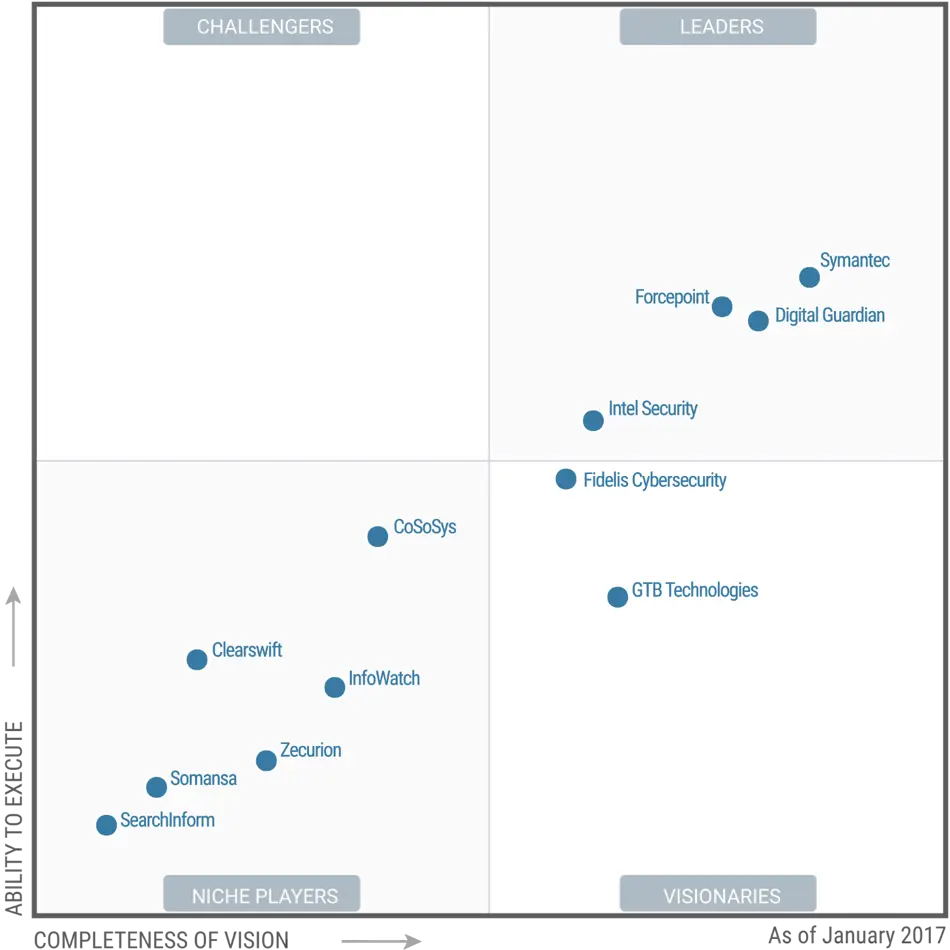
\includegraphics[width=.7\textwidth, height=.6\textheight, keepaspectratio]{2017-gartner-magic-quadrant-for-enterprise-data-loss-prevention-new.png}}
        \caption{Quadrante magico di Gartner}\label{Gartner}
      \end{figure}

\section{Accenni sul progetto}
Il progetto implementato consiste in una soluzione DLP per la protezione dei dati in transito, più precisamente per
l'identificazione di eventuali dati riservati presenti nelle email aziendali, in modo da prevenirne la perdita
ed evitarne la diffusione.

Il confronto effettuato tra i prodotti principali presenti sul mercato, anche se nessuno di essi è stato utilizzato 
ai fini del progetto, è risultato utile per capire quali caratteristiche dovesse possedere la soluzione DLP implementata.

\section{Tecnologie utilizzate per il progetto}
Per l'implementazione del progetto sono state utilizzate diverse tecnologie:
    \subsection{Postfix}
    Postfix è un server di posta open source scritto in C da Wietse Zweitze Venema e distribuito con licenza IBM 
    Public License. Nasce alla fine degli anni '90 con lo scopo di fornire un'alternativa a Sendmail che offrisse 
    maggiori garanzie per quanto riguarda la sicurezza \cite{Postfix1}.
    Dato che il capitolo 5 si concentra esclusivamente su Postfix e come è stato utilizzato per implementare la 
    soluzione DLP, non verranno dati ulteriori dettagli in questo paragrafo.
    
    \subsection{Python}
    Python è un linguaggio di programmazione ad alto livello che si presta ad essere utilizzato in ambito didattico per la sua semplicità. È orientato a oggetti, adatto, tra gli altri usi, a sviluppare 
    degli script \cite{Python1}. A differenza di linguaggi come il C e Java è un linguaggio interpretato e non compilato. 
    I programmi scritti in Python sono portabili, 
    cioè possono essere eseguiti su differenti sistemi operativi, tra i quali Windows, Mac OS X e GNU/Linux. 
    Inoltre è gratuito e open source, utilizzabile da chiunque \cite{boscaini2017imparare}.

    
    \subsection{Bash}
    La Bash è la shell più diffusa e utilizzata in ambiente Linux. 
    Si tratta di un interprete di comandi che permette all'utente di comunicare col sistema operativo attraverso una
    serie di funzioni predefinite, o di eseguire programmi e script.
    Bash mette a disposizione un semplice linguaggio di scripting nativo che permette di svolgere compiti 
    più complessi, non solo raccogliendo in uno script una serie di comandi, 
    ma anche utilizzando variabili, funzioni e strutture di controllo di flusso \cite{Bash1}.
    
    \subsection{Apache Tika}
    Apache tika è un tool per l’analisi dei contenuti, permette di estrarre il testo da migliaia di tipi di file diversi \cite{tika}.
    Libreria utile per estrarre il testo dagli allegati delle email per verificare se contengono dati riservati. 
    %Ho utilizzato questa libreria all’interno del mio script Python per estrapolare il testo dai file allegati 
    %alle email in modo da verificare la presenza di dati sensibili.
    
    \subsection{Virtualbox}
    Oracle VM VirtualBox è un software gratuito e open source per l'esecuzione di macchine virtuali \cite{VirtualBox1}.
    L'uso di questo software ha reso possibile l'installazione del sistema operativo CentOS 8 
    (distribuzione Linux derivata da Red Hat Enterprise Linux), che ha ospitato il mail server Postfix.

    \chapter{Progettazione}

\section{Analisi}
  Questo capitolo ha come obiettivo quello di descrivere tutte le funzionalità che deve soddisfare la 
  soluzione DLP e gli eventuali vincoli a cui deve attenersi.

  \subsection{Soluzione DLP per il traffico email}
  Tenuto conto del modello ISACA,

  La soluzione DLP da implementare consisterà nella protezione dei data-in-motion, più nello specifico
  andrà a focalizzarsi sulla protezione delle email. La soluzione andrà a monitorare il traffico email e
  il loro contenuto in modo da:

  \begin{enumerate}
      \item {identificare la presenza di dati sensibili al loro interno;}
      \item {prevenire la loro perdita / 
      invio (in modo da prevenire la fuoriuscita dall’ambiente aziendale di queste informazioni).}
  \end{enumerate}

  \subsection{Motivazione scelta e obiettivo}
  La scelta di implementare questa funzionalità è dovuta al fatto che le email sono uno, 
  se non il principale, dei metodi di comunicazione in ambito aziendale.
  L’implementazione di questa funzionalità, oltre ad essere utile, risulta anche interessante.

  Lo scopo principale è quello di incrementare la sicurezza enterprise,  
  evitando la diffusione di dati sensibili.

  \pagebreak
  \subsection{Glossario}

  \begin{table}[!b]
      \centering
      \resizebox{\textwidth}{!}{%
      \begin{tabular}{|l|l|}
      \hline
      \rowcolor[HTML]{EFEFEF} 
      \textbf{Termine} &
        \textbf{Definizione} \\ \hline 
      Dipendente &
        \begin{tabular}[c]{@{}l@{}}Membro del personale. \\ Può essere il mittente o \\ il destinatario di una email.\end{tabular} \\ \hline 
      Mittente &
        \begin{tabular}[c]{@{}l@{}}Colui che invia la email.\\ Per questo progetto il mittente \\ è inteso come un dipendente \\ interno all’azienda.\end{tabular} \\ \hline
      Destinatario &
        \begin{tabular}[c]{@{}l@{}}Colui che riceve la email.\\ Può essere sia interno che \\ esterno all’azienda.\end{tabular} \\ \hline
      Email &
        \begin{tabular}[c]{@{}l@{}}Oggetto che va monitorato e \\ ispezionato dalla soluzione DLP.\\ In generale una email contiene:\\ -  Mittente;\\ -  Destinatario;\\ -  Oggetto;\\ -  Corpo;\\ -  Allegato (opzionale).\\ \\ I primi due attributi possono \\ essere oggetto di analisi del contesto, \\ mentre gli ultimi tre verranno ispezionati \\ durante l’analisi del contenuto.\end{tabular} \\ \hline
      Dati sensibili &
        \begin{tabular}[c]{@{}l@{}}Dati che hanno maggior valore, ad esempio:\\ - dati di business\\  (contratti, proprietà intellettuale, progetti);\\  \\ - dati personali \\ (Codici fiscali, date di nascita \\ e altre informazioni sui dipendenti \\ e/o clienti);\\ \\ - dati finanziari \\ (dati della carta di credito o di altre modalità di pagamento);\\ eccetera.\end{tabular} \\ \hline
      \end{tabular}%
      }
      \caption{Glossario dei termini}\label{Glossario}
      \end{table}

      \pagebreak
      
      \subsection{Analisi dei requisiti}

        \subsubsection{Obiettivo utente:}
        La soluzione DLP deve identificare la presenza di dati/documenti sensibili all’interno delle email 
        in modo da evitare che lascino il sistema aziendale.

        \subsubsection{Requisiti funzionali:}



        \begin{table}[htp]
            \centering
            \resizebox{\textwidth}{!}{%
            \begin{tabular}{ll}
            \multicolumn{2}{l}{requisito funzionale 1 (RF01): \textbf{Monitoraggio traffico SMTP}}                               \\ \hline
            \rowcolor[HTML]{EFEFEF} 
            \multicolumn{1}{|l|}{\cellcolor[HTML]{EFEFEF}ID}       & \multicolumn{1}{l|}{\cellcolor[HTML]{EFEFEF}RF01}           \\ \hline
            \multicolumn{1}{|l|}{Nome}                             & \multicolumn{1}{l|}{Monitoraggio traffico email (SMTP)}     \\ \hline
            \rowcolor[HTML]{EFEFEF} 
            \multicolumn{1}{|l|}{\cellcolor[HTML]{EFEFEF}Definizione} &
              \multicolumn{1}{l|}{\cellcolor[HTML]{EFEFEF}La soluzione deve monitorare il traffico email} \\ \hline
            \multicolumn{1}{|l|}{Motivazione} &
              \multicolumn{1}{l|}{\begin{tabular}[c]{@{}l@{}}Senza l'implementazione di questo requisito,\\ la soluzione non può funzionare. È il requisito\\ base per poter implementare gli altri\end{tabular}} \\ \hline
            \rowcolor[HTML]{EFEFEF} 
            \multicolumn{1}{|l|}{\cellcolor[HTML]{EFEFEF}Priorità} & \multicolumn{1}{l|}{\cellcolor[HTML]{EFEFEF}Indispensabile} \\ \hline
            \multicolumn{1}{|l|}{Dipendenze}                       & \multicolumn{1}{l|}{/}                                      \\ \hline
            \end{tabular}%
            }
            \newline
            \vspace*{1 cm}
            \newline
        \end{table}



        \begin{table}[htp]
            \centering
            \resizebox{\textwidth}{!}{%
            \begin{tabular}{ll}
            \multicolumn{2}{l}{requisito funzionale 2 (RF02): \textbf{Analisi del contenuto}}                                    \\ \hline
            \rowcolor[HTML]{EFEFEF} 
            \multicolumn{1}{|l|}{\cellcolor[HTML]{EFEFEF}ID}       & \multicolumn{1}{l|}{\cellcolor[HTML]{EFEFEF}RF02}           \\ \hline
            \multicolumn{1}{|l|}{Nome}                             & \multicolumn{1}{l|}{Analisi del contenuto}                  \\ \hline
            \rowcolor[HTML]{EFEFEF} 
            \multicolumn{1}{|l|}{\cellcolor[HTML]{EFEFEF}Definizione} &
              \multicolumn{1}{l|}{\cellcolor[HTML]{EFEFEF}\begin{tabular}[c]{@{}l@{}}La soluzione deve analizzare il contenuto di\\ ogni email che viene inviata.\end{tabular}} \\ \hline
            \multicolumn{1}{|l|}{Motivazione} &
              \multicolumn{1}{l|}{\begin{tabular}[c]{@{}l@{}}Senza l'implementazione di questo requisito,\\ La soluzione non sarebbe in grado di\\ \\ identificare contenuti sensibili\end{tabular}} \\ \hline
            \rowcolor[HTML]{EFEFEF} 
            \multicolumn{1}{|l|}{\cellcolor[HTML]{EFEFEF}Priorità} & \multicolumn{1}{l|}{\cellcolor[HTML]{EFEFEF}Indispensabile} \\ \hline
            \multicolumn{1}{|l|}{Dipendenze}                       & \multicolumn{1}{l|}{RF01}                                   \\ \hline
            \end{tabular}%
            }
            \end{table}


        \begin{table}[htp]
            \centering
            \resizebox{\textwidth}{!}{%
            \begin{tabular}{ll}
            \multicolumn{2}{l}{requisito funzionale 3 (RF03): \textbf{Analisi del contesto}}                                                   \\ \hline
            \rowcolor[HTML]{EFEFEF} 
            \multicolumn{1}{|l|}{\cellcolor[HTML]{EFEFEF}ID}       & \multicolumn{1}{l|}{\cellcolor[HTML]{EFEFEF}RF03}                         \\ \hline
            \multicolumn{1}{|l|}{Nome}                             & \multicolumn{1}{l|}{Analisi del contesto}                                 \\ \hline
            \rowcolor[HTML]{EFEFEF} 
            \multicolumn{1}{|l|}{\cellcolor[HTML]{EFEFEF}Definizione} &
              \multicolumn{1}{l|}{\cellcolor[HTML]{EFEFEF}\begin{tabular}[c]{@{}l@{}}La soluzione, oltre ad analizzare il contenuto\\ di una email, deve anche tenere conto del \\ contesto\end{tabular}} \\ \hline
            \multicolumn{1}{|l|}{Motivazione} &
              \multicolumn{1}{l|}{\begin{tabular}[c]{@{}l@{}}Effettuare l'analisi del contesto può essere un\\ utile supporto all'analisi del contenuto.\end{tabular}} \\ \hline
            \rowcolor[HTML]{EFEFEF} 
            \multicolumn{1}{|l|}{\cellcolor[HTML]{EFEFEF}Priorità} & \multicolumn{1}{l|}{\cellcolor[HTML]{EFEFEF}Non Indispensabile, ma utile} \\ \hline
            \multicolumn{1}{|l|}{Dipendenze}                       & \multicolumn{1}{l|}{RF01}                                                 \\ \hline
            \end{tabular}%
            }
            \end{table}



        \begin{table}[htp]
            \centering
            \resizebox{\textwidth}{!}{%
            \begin{tabular}{ll}
            \multicolumn{2}{l}{requisito funzionale 4 (RF04): \textbf{Identificazione dati sensibili}}                   \\ \hline
            \rowcolor[HTML]{EFEFEF} 
            \multicolumn{1}{|l|}{\cellcolor[HTML]{EFEFEF}ID}       & \multicolumn{1}{l|}{\cellcolor[HTML]{EFEFEF}RF04}           \\ \hline
            \multicolumn{1}{|l|}{Nome}                             & \multicolumn{1}{l|}{Identificazione di contenuti sensibili} \\ \hline
            \rowcolor[HTML]{EFEFEF} 
            \multicolumn{1}{|l|}{\cellcolor[HTML]{EFEFEF}Definizione} &
              \multicolumn{1}{l|}{\cellcolor[HTML]{EFEFEF}\begin{tabular}[c]{@{}l@{}}La soluzione dev'essere in grado di identificare eventuali\\ dati/contenuti sensibili presenti all'interno delle email\end{tabular}} \\ \hline
            \multicolumn{1}{|l|}{Motivazione} &
              \multicolumn{1}{l|}{\begin{tabular}[c]{@{}l@{}}Senza l'implementazione di questo requisito non è \\ possibile raggiungere l'obiettivo utente\end{tabular}} \\ \hline
            \rowcolor[HTML]{EFEFEF} 
            \multicolumn{1}{|l|}{\cellcolor[HTML]{EFEFEF}Priorità} & \multicolumn{1}{l|}{\cellcolor[HTML]{EFEFEF}Indispensabile} \\ \hline
            \multicolumn{1}{|l|}{Dipendenze}                       & \multicolumn{1}{l|}{RF01, RF02}                             \\ \hline
            \end{tabular}%
            }
            \end{table}


        \begin{table}[htp]
            \centering
            \resizebox{\textwidth}{!}{%
            \begin{tabular}{ll}
            \multicolumn{2}{l}{requisito funzionale 5 (RF05): \textbf{Azioni di risposta}}                         \\ \hline
            \rowcolor[HTML]{EFEFEF} 
            \multicolumn{1}{|l|}{\cellcolor[HTML]{EFEFEF}ID}       & \multicolumn{1}{l|}{\cellcolor[HTML]{EFEFEF}RF05}           \\ \hline
            \multicolumn{1}{|l|}{Nome}                             & \multicolumn{1}{l|}{Intraprendere azioni di risposta}       \\ \hline
            \rowcolor[HTML]{EFEFEF} 
            \multicolumn{1}{|l|}{\cellcolor[HTML]{EFEFEF}Definizione} &
              \multicolumn{1}{l|}{\cellcolor[HTML]{EFEFEF}\begin{tabular}[c]{@{}l@{}}La soluzione deve poter intraprendere una varietà di azioni:\\ 1. consentire l’invio;\\ 2. bloccare l’invio;\\ 3. eliminare il contenuto sensibile e procedere con l’invio.\end{tabular}} \\ \hline
            \multicolumn{1}{|l|}{Motivazione} &
              \multicolumn{1}{l|}{\begin{tabular}[c]{@{}l@{}}Poiché la soluzione deve evitare che documenti sensibili \\ lascino il sistema aziendale, l'implementazione di questo \\ requisito è fondamentale\end{tabular}} \\ \hline
            \rowcolor[HTML]{EFEFEF} 
            \multicolumn{1}{|l|}{\cellcolor[HTML]{EFEFEF}Priorità} & \multicolumn{1}{l|}{\cellcolor[HTML]{EFEFEF}Indispensabile} \\ \hline
            \multicolumn{1}{|l|}{Dipendenze}                       & \multicolumn{1}{l|}{RF01, RF04}                             \\ \hline
            \end{tabular}%
            }
            \end{table}


        \begin{table}[htp]
        \centering
        \resizebox{\textwidth}{!}{%
        \begin{tabular}{ll}
        \multicolumn{2}{l}{requisito funzionale 6 (RF06): \textbf{Avviso in caso di blocco}}                                 \\ \hline
        \rowcolor[HTML]{EFEFEF} 
        \multicolumn{1}{|l|}{\cellcolor[HTML]{EFEFEF}ID}       & \multicolumn{1}{l|}{\cellcolor[HTML]{EFEFEF}RF06}           \\ \hline
        \multicolumn{1}{|l|}{Nome}                             & \multicolumn{1}{l|}{Avviso in caso di blocco}               \\ \hline
        \rowcolor[HTML]{EFEFEF} 
        \multicolumn{1}{|l|}{\cellcolor[HTML]{EFEFEF}Definizione} &
          \multicolumn{1}{l|}{\cellcolor[HTML]{EFEFEF}\begin{tabular}[c]{@{}l@{}}La soluzione deve sempre avvisare il mittente \\ in caso decida di bloccare l'invio della \\ email\end{tabular}} \\ \hline
        \multicolumn{1}{|l|}{Motivazione} &
          \multicolumn{1}{l|}{\begin{tabular}[c]{@{}l@{}}Utile avvisare il mittente in caso\\ sia necessario bloccare l'invio della sua email\end{tabular}} \\ \hline
        \rowcolor[HTML]{EFEFEF} 
        \multicolumn{1}{|l|}{\cellcolor[HTML]{EFEFEF}Priorità} & \multicolumn{1}{l|}{\cellcolor[HTML]{EFEFEF}Indispensabile} \\ \hline
        \multicolumn{1}{|l|}{Dipendenze}                       & \multicolumn{1}{l|}{RF05}                                   \\ \hline
        \end{tabular}%
        }
        \newline
        \vspace*{1 cm}
        \newline
        \end{table}

        \pagebreak
        \subsection{Dipendenze tra requisiti}
        Di seguito ho stilato un elenco delle dipendenze formatesi tra i requisiti.
        La nomenclatura utilizzata è la seguente:
        \begin{flushleft}
          x -> y: il requisito x dipende dal requisito y
          \newline
          \newline
          RF02 -> RF01

          RF03 -> RF01

          RF04 -> RF01, RF02

          RF05 -> RF01, RF04

          RF06 -> RF05
          \newline
          \newline
          Elenco delle dipendenze semplificato: 
          \newline
          \newline
          RF02 -> RF01

          RF03 -> RF01

          RF04 -> RF02

          RF05 -> RF04 
          
          RF06 -> RF05
        \end{flushleft}

        \newpage
        \subsection{Grafo delle Dipendenze}
        Le dipendenze tra i requisiti formano un grafo aciclico che bisogna tenere in considerazione in caso si debba modificare uno dei requisiti del sistema.

        \begin{figure}[htp]
          \centering
          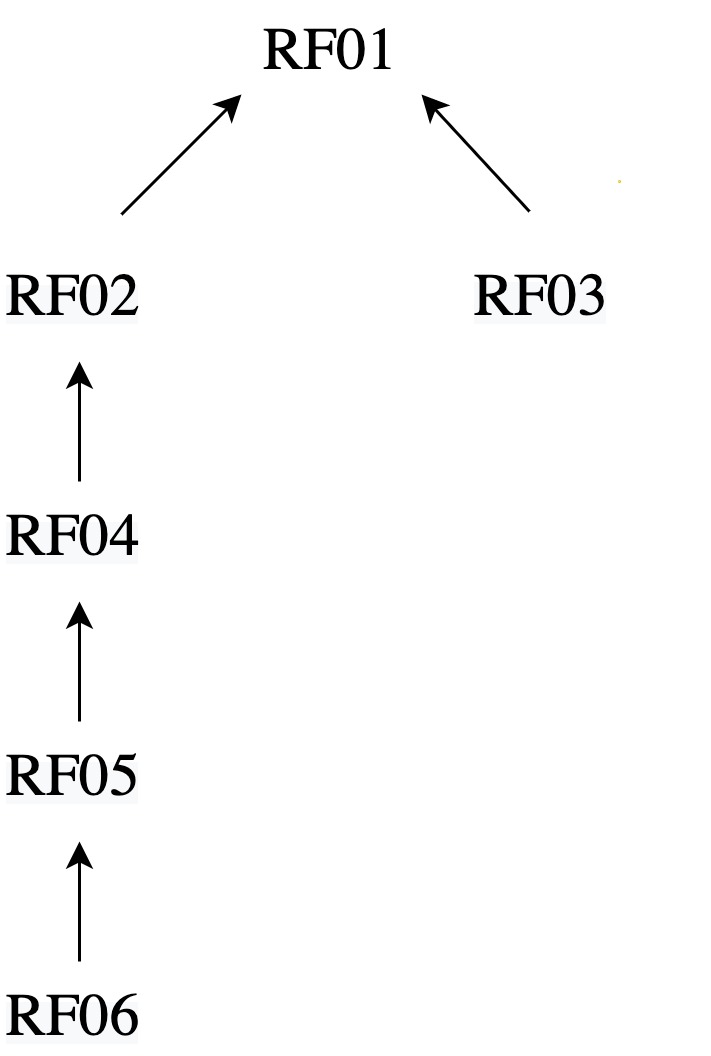
\includegraphics[width=.4\textwidth, height=.3\textheight, keepaspectratio]{grafo.jpg}
          \caption{Grafo aciclico delle dipendenze}\label{grafoDipendenze}
        \end{figure}

\section{Disegno dell'architettura}

  Per la progettazione della soluzione inseriremo la nostra soluzione DLP
  tra il mail client (Outlook) e il mail server aziendale (Aruba). La soluzione DLP deciderà se lasciar 
  passare l' email verso il mail server aziendale, oppure bloccarne l'invio.
  \begin{figure}[htp]
    \centering
    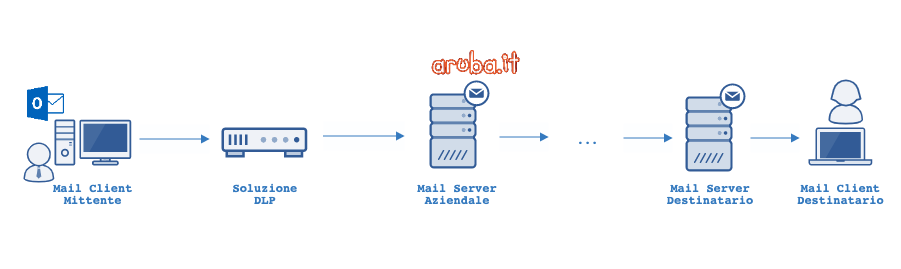
\includegraphics[width=12cm, height=16cm, keepaspectratio]{disegno1.png}
    \caption{disegno architettura per un mail client}\label{disegno1}
  \end{figure}

  \pagebreak
  La soluzione DLP verrà implementata attraverso l'uso di un mail server di inoltro (relay mail server).
  Il disegno subirà una piccola modifica.

  \begin{figure}[htp]
    \centering
    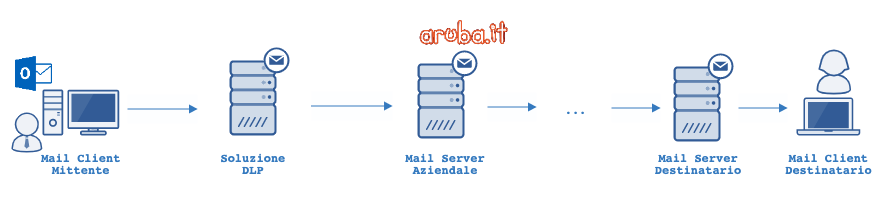
\includegraphics[width=12cm, height=16cm, keepaspectratio]{disegno2.png}
    \caption{soluzione DLP attraverso mail server di relay}\label{disegno2}
  \end{figure}

  Come ultimo passo andremo a considerare una sottorete composta dagli host dei dipendenti dell'azienda, al
  posto di un unico client. Questa è la configurazione che più rispecchia la realtà.

  \begin{figure}[htp]
    \centering
    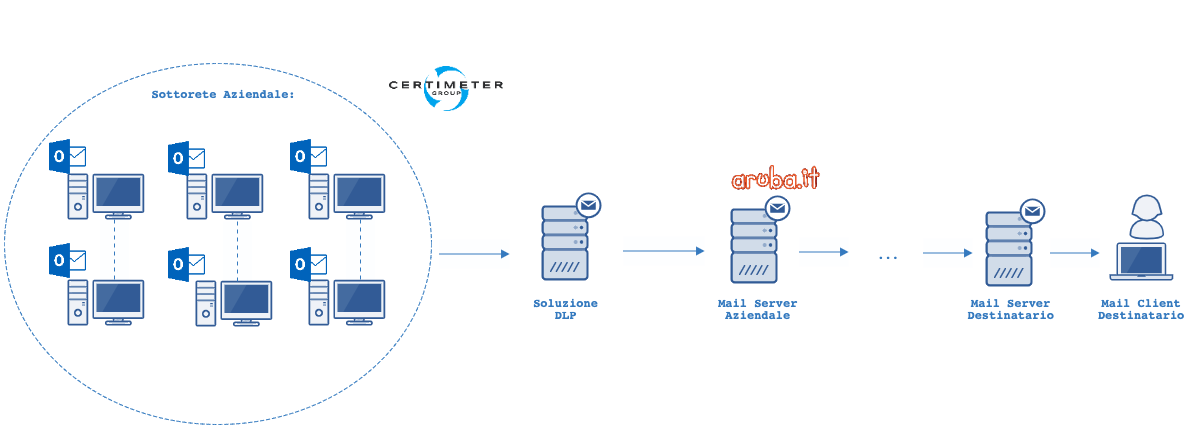
\includegraphics[width=12cm, height=16cm, keepaspectratio]{disegno3.png}
    \caption{soluzione DLP attraverso mail server di relay}\label{disegno3}
  \end{figure}

  \subsection{Descrizione del flusso di dati e di controllo}
  Come mostrato dalla figure \ref{disegno2} e \ref{disegno3}, Quando un dipendente invia una email, questa
  passerà dal relay mail server che deciderà se bloccarla, oppure inoltrarla al mail server aziendale. L'email
  continuerà il suo cammino fino ad arrivare al mail server del destinatario. A quel punto potrà essere scaricata
  dal mail client del destinatario.

    \chapter{Postfix}

\begin{figure}[htp]
    \centering
    
\includegraphics[width=4cm, height=8cm, keepaspectratio]{logo_postfix.png}
        \caption{logo di Postfix}\label{logoPostfix}
  \end{figure}

  Questo capitolo è totalmente incentrato su Postfix, descrivendone il funzionamento, 
  l'architettura e come è stato utilizzato per soddisfare i requisiti scoperti durante la fase di analisi.
  
  Come accennato nel capitolo 3, la soluzione DLP è stata implementata attraverso l'utilizzo di un 
  mail server configurato in modalità di inoltro.
  La scelta sul prodotto migliore da utilizzare è ricaduta tra Sendmail e Postfix. 
  Sendmail è stato l'MTA più diffuso tra i sistemi UNIX, ma ormai sono stati riscontrati problemi in materia
  di sicurezza. 
  Per questo motivo è stato deciso di utilizzare Postfix, un software nato con l'obiettivo di sostituire Sendmail. Il passaggio
  tra i due è piuttosto semplice dato che Postfix è stato progettato in modo da essere compatibile con il 
  suo predecessore.
  A differenza dei prodotti DLP trattati nel capitolo 3, sia Sendmail che Postfix sono software open source e
  quindi hanno rappresentato un'ottima soluzione per lo sviluppo di questo progetto.
  La figura \ref{logoPostfix} mostra il logo di Postfix.
  Nel prossimo paragrafo viene presentata un'introduzione su Postfix e sulla sua architettura. Per ulteriori
  informazioni è possibile consultare il sito ufficiale al seguente indirizzo: \url{http://www.postfix.org/}
   
  \pagebreak
  \section{Introduzione di Postfix}
  Postfix è un mail server che trasporta messaggi di posta elettronica da un mail client 
  (o da un altro mail server) verso un server di posta remoto, o in locale. 
  Per lo sviluppo della soluzione DLP è stato utilizzato come client di posta ufficiale Outlook 
  ed è stato configurato Postifix come mail server di inoltro, 
  così da inoltrare le email verso il server di posta elettronica aziendale Aruba. 
  Una delle funzionalità particolarmente interessanti che offre Postfix è quella di effettuare 
  un’analisi sul contenuto delle email (durante la descrizione della fase di implementazione viene illustrato 
  come è stato configurato il controllo dei contenuti e vengono descritti alcuni filtri sviluppati).
  
  \subsection{Architettura di Postfix}
  Il vantaggio principale che ha portato Postfix a diventare l’erede di Sendmail, oltre la compatibilità, 
  è la sicurezza. Postfix è stato progettato in modo da essere dotato di un’architettura modulare. 
  È composto da diversi demoni, ognuno dei quali svolge un preciso compito ed esegue con i privilegi minimi 
  necessari per portarlo a termine. Il  \textit{master} è l’unico processo che esegue con i privilegi di root
  e rimane sempre attivo. 
  La funzione principale del \textit{master} è quella di gestire tutti gli altri processi. 
  I processi non hanno legami di parentela con i processi utente, quindi sono immuni da vulnerabilità che 
  coinvolgono la relazione padre-figlio. Per questo motivo Postfix non è vulnerabile da attacchi che sfruttano 
  l’interprocess communication, come ad esempio l’invio di segnali o l’utilizzo della memoria condivisa. 
  Postfix è immune anche da attacchi di tipo Buffer Overflow. 
  In caso di mancanza di risorse è progettato per rallentare i suoi compiti, facendosi da parte in modo che 
  il sistema si possa riprendere, rendendo meno efficienti gli attacchi DOS nei suoi confronti.
  
  La ricezione dei messaggi può avvenire in due modi: localmente, oppure tramite la rete \cite{hildebrandt2005book}.
  
  \subsection{Ricezione locale dei messaggi}\label{sec:ricezioneLocale}
  La ricezione locale di email può avvenire, ad esempio, quando si invia un messaggio da terminale 
  (dallo stesso host che ospita il server Postfix) utilizzando il comando \textit{sendmail}. 
  
  I messaggi locali sono depositati nella cartella maildrop dal comando \textit{postdrop} di Postfix. 
  Postdrop non fa altro che creare un file all’interno della cartella maildrop copiandone all’interno 
  l’input passato al comando (stdin, che corrisponde all'email inviata localmente). 
  
  Il demone \textit{pickup} a questo punto preleva il messaggio dalla cartella (coda) maildrop e lo 
  invia al demone \textit{cleanup}. 
  Questo è il demone incaricato di effettuare i controlli sul contenuto che come già detto sono documentati 
  nel capitolo 6. 
  Una volta che l’email supera i controlli, questa finisce nella coda dei messaggi in arrivo, passando 
  sotto il controllo del gestore delle code (\textit{qmgr}).

  In questo caso, poiché Postfix è stato configurato come relay mail server, 
  \textit{qmgr} contatterà il demone \textit{smtp} per inviare il messaggio al next-hop. In caso si dovesse consegnare 
  il messaggio localmente verrebbe contattato \textit{local} e nel caso lo si dovesse passare ad un comando, 
  verrebbe richiamato il demone \textit{pipe} \cite{Postfix2}.
  
  \subsection{Ricezione dei messaggi dalla rete}
  I messaggi ricevuti dalla rete sono accettati dal demone \textit{smtpd}. Una volta ricevuto il messaggio, 
  \textit{smtpd} provvede a consegnarlo a \textit{cleanup} e da quel momento la strada percorsa 
  è la stessa di quella effettuata dalle email ricevute in locale.
  La configurazione effettuata per la soluzione DLP consiste in una variante di questa opzione.
  I messaggi ricevuti dalla rete, una volta controllati da \textit{cleanup}
  e tornati sotto il controllo di \textit{qmgr}, vengono passati al demone \textit{pipe} 
  per essere consegnati allo script esterno ed esaminati.
  Se non vengono trovati dati riservati, viene utilizzato il comando \textit{sendmail} per riconsegnare 
  il messaggio a Postfix. 
  Una volta fatto questo, Postfix vede il messaggio come ricevuto in locale, quindi, da quel momento in poi, 
  vale quanto detto nel paragrafo \ref{sec:ricezioneLocale}.
  
  \subsection{Rifiuto di un messaggio}
  Quando Postfix decide di rifiutare un messaggio, ad esempio perché vengono identificati dati riservati, 
  il demone \textit{bounce} provvede ad avvisare il mittente, includendo opzionalmente una motivazione del perché non
  sia stato possibile accettare e quindi consegnare il messaggio.
  
  \section{Utilizzo di Postfix come soluzione DLP}
  In questo paragrafo vengono richiamati i requisiti descritti durante la fase di analisi e 
  viene illustrato come possono essere soddisfatti attraverso l'utilizzo di Postfix. In particolare la tabella
  \ref{PostfixDLP} stila un elenco dei requisiti nella colonna di sinistra, mentre alla destra di ognuno viene illustrato
  cosa offre Postfix per poterlo soddisfare.
  
   
  
  \begin{table}[htp]
      \centering
      \resizebox{\textwidth}{!}{%
      \begin{tabular}{|l|l|}
      \hline
      \rowcolor[HTML]{EFEFEF} 
      \textbf{1. Monitoraggio traffico email} &
        \begin{tabular}[c]{@{}l@{}}Poiché si utilizza un mail server di relay,\\ questo requisito risulta soddisfatto.\end{tabular} \\ \hline
      \textbf{2. Analisi del contenuto} &
        \begin{tabular}[c]{@{}l@{}}Postfix permette di analizzare:\\ - l'oggetto del messaggio;\\ - il corpo del messaggio;\\ - l'allegato di un messaggio;\\ \\ l'analisi avviene mediante l'utilizzo di \\ espressioni regolari.\\ Postfix non offre la possibilità di \\ analizzare il contenuto di un allegato, ma \\ permette di applicare delle regole per \\ filtrare in base al filename e all'estensione.\end{tabular} \\ \hline
      \rowcolor[HTML]{EFEFEF} 
      \textbf{3. Analisi del contesto} &
        \begin{tabular}[c]{@{}l@{}}È possibile effettuare un'analisi degli\\ header del messaggio. Si possono\\ effettuare delle restrizioni in base al\\ mittente e destinatario o in base ad un \\ dominio.\\ \\ alcuni header d'interesse: \\ - FROM:\\ - TO:\end{tabular} \\ \hline
      \textbf{\begin{tabular}[c]{@{}l@{}}4. Identificazione di dati     riservati\end{tabular}} &
        \begin{tabular}[c]{@{}l@{}}L'identificazione di dati/contenuti riservati\\ è possibile per mezzo dell'analisi del \\ contenuto.\end{tabular} \\ \hline
      \rowcolor[HTML]{EFEFEF} 
      \textbf{5. Intraprendere azioni di risposta} &
        \begin{tabular}[c]{@{}l@{}}Azioni di risposta offerte da Postfix:\\ 1. REJECT;\\ 2. IGNORE;\\ 3. WARN;\\ 4. HOLD;\\ 5. DISCARD;\\ 6. FILTER;\\ 7. REDIRECT.\\ \\ Nel paragrafo successivo viene spiegato il \\ funzionamento di ogni voce citata.\end{tabular} \\ \hline
      \textbf{6. Avviso in caso di blocco} &
        \begin{tabular}[c]{@{}l@{}}Nel caso in cui un messaggio di posta \\ non dovesse essere accettato da Postfix\\ (per mezzo della clausola REJECT), \\ verrà notificato il mittente.\end{tabular} \\ \hline
      \end{tabular}%
      }
      \caption{Utilizzo di Postfix come soluzione DLP}\label{PostfixDLP}
      \end{table}
  
  
  
  \begin{table}[htp]
    \subsection{Azioni di risposta di Postfix}
  \begin{enumerate}[label=\textbf{\arabic*})]
      \item{\textbf{REJECT [testo opzionale]:}}\\
      Nel caso in cui venga definita la clausola REJECT, Postfix non accetta il messaggio 
      da consegnare (ne blocca l'invio).
      [testo opzionale] è consegnato al client che ha cercato di inviare il messaggio.
      L'evento viene tracciato nei log (insieme al motivo [testo opzionale]).
  
      \item{\textbf{IGNORE:}}\\
      Se definita la clausola IGNORE, Postfix rimuove le righe del messaggio che fanno match con 
      le espressioni regolari definite. Elimina i dati riservati e poi procede con l'inoltro del 
      messaggio.
      
      \item{\textbf{WARN [testo opzionale]:}}\\
      Definendo una regola con la parola chiave WARN, il mittente è in grado di inviare il messaggio di 
      posta. Nei log viene generato un warning contenente [testo opzionale].
      
      \item{\textbf{HOLD [testo opzionale]: (Quarantena del messaggio)}}\\
      L'opzione HOLD mantiene il messaggio nella hold queue di Postfix in quarantena. Questa funzionalità
      è utilizzata quando è necessario l'intervento umano. Il compito di decidere le sorti del messaggio
      ricade sull'analista DLP, o postmaster se si vuole utilizzare la terminologia di Postfix. A questo punto
      il messaggio viene sbloccato, oppure eliminato.
      Nei log viene tracciata la riga che ha fatto match con la regola definita e se specificato viene incluso
      anche [testo opzionale].
      
      
      \item{\textbf{DISCARD [testo opzionale]:}}\\
      Postfix offre anche l'opzione DISCARD. Quando è specificata questa opzione, lato mittente il 
      messaggio di posta risulta consegnato correttamente. Invece di trasportarlo verso la destinazione finale, 
      Postfix silenziosamente lo elimina.
      Se definito [testo opzionale], viene tracciato nei log insieme alla riga che ha fatto match con la regola 
      specificata. 
      
      \item{\textbf{FILTER [testo opzionale]:}}
      Questa opzione invia il messaggio ad un filtro esterno. Molto utilizzato per effettuare scansioni 
      antivirus e antispam.
      
      \item{\textbf{REDIRECT user@dominio.it:}} 
      L'ultima opzione è quella di REDIRECT e, come si può intuire dalla parola, instrada il messaggio al 
      destinatario specificato, anziché inviarlo a quello originale \cite{hildebrandt2005book}.
  \end{enumerate}
  \end{table}
  
  \pagebreak
  \begin{table}[htp]
    \subsection{Gestione dei messaggi in quarantena}
    Il demone incaricato di gestire le code è \textit{qmgr}. \textit{qmgr} getisce cinque code:
    \begin{itemize}
      \item incoming
      \item active
      \item deferred
      \item hold
      \item corrupt
    \end{itemize}
  \end{table}
  
  Tutti i messaggi in ingresso e in uscita passano attraverso \textit{qmgr}. 
  A scopo progettuale, è oggetto di focus soltanto la coda di hold, 
  quella dove si trovano i messaggi bloccati in quarantena.
  
  Postfix mette a disposizione dei comandi per permettere al postmaster, manualmente, di gestire i messaggi che si 
  trovano in coda.
  
  \subsubsection{Visualizzazione dei messaggi in coda}
  Attraverso il comando \textit{postqueue -p} oppure \textit{mailq} (tenuto per compatibilità con Sendmail) è possibile visualizzare tutti
  i messaggi in coda. È importante notare che i messaggi che si trovano nella hold queue presentano accanto al Queue ID 
  un punto esclamativo.
  
  \begin{verbatim}
  [root@localhost palfag]# mailq
  -Queue ID-  --Size-- ----Arrival Time---- -Sender/Recipient-------
  4B5D58E9F44!     638 Fri May 21 11:36:57  paolo.fagioli@certimeter.it
                                            palfag33@gmail.com
  
  -- 0 Kbytes in 1 Request.
  \end{verbatim}
  
  \newpage
  \subsubsection{Ispezione di un messaggio in coda}
  Per decidere se consentire l'invio o il blocco del messaggio, il postmaster deve esaminarne il contenuto, 
  quest'azione è possibile utilizzando il comando \textit{postcat -q <Queue\_ID>}.

  \begin{verbatim}
  [root@localhost palfag]# postcat -q 4B5D58E9F44 

  *** MESSAGE CONTENTS hold/4B5D58E9F44 ***
  Received: from [192.168.8.109] (_gateway [10.0.2.2])
  by mail.palfag.it (Postfix) with ESMTPSA id 4B5D58E9F44
  for <palfag33@gmail.com>; Fri, 21 May 2021 11:36:57 +0200 (CEST)
  User-Agent: Microsoft-MacOutlook/16.49.21050901
  Date: Fri, 21 May 2021 11:37:09 +0200
  Subject: Contenuto privato
  From: Paolo Fagioli <paolo.fagioli@certimeter.it>
  To: Paolo Fagioli <palfag33@gmail.com>
  Message-ID: <907A6E2B-235A-43C1-A986-3ACA372BC101@certimeter.it>
  Thread-Topic: Contenuto privato
  Mime-version: 1.0
  Content-type: text/plain;
  charset="UTF-8"
  Content-transfer-encoding: 7bit

  Caro Paolo,
  tutto bene?

  Saluti da me stesso
  \end{verbatim}
  
  
  \subsubsection{Eliminazione di un messaggio dalla coda}
  Per eliminare un messaggio dalla coda si utilizza il comando \textit{postsuper -d <Queue\_ID>}.
  \textit{postsuper -d ALL} elimina tutti i messaggi dalla coda.

  \begin{verbatim}
  [root@localhost palfag]# mailq
  -Queue ID-  --Size-- ----Arrival Time---- -Sender/Recipient-------
  4B5D58E9F44!     638 Fri May 21 11:36:57  paolo.fagioli@certimeter.it
                                            palfag33@gmail.com
  
  -- 0 Kbytes in 1 Request.
  [root@localhost palfag]# postsuper -d 4B5D58E9F44 
  postsuper: 4B5D58E9F44: removed
  postsuper: Deleted: 1 message
  [root@localhost palfag]# mailq
  Mail queue is empty
  \end{verbatim}
  
  
  \subsubsection{Consenso all'invio di un messaggio}
  I messaggi che finiscono in quarantena, senza l'intervento umano, sono destinati a rimanere nella hold queue per una 
  quantità di tempo indefinita. Se il postmaster decide di lasciar passare il messaggio deve utilizzare il comando
  \textit{postsuper -H <Queue\_ID>}. In questo modo il messaggio con id == Queue\_ID può lasciare la coda di hold 
  tornando sotto il controllo del gestore delle code, 
  che può rischedulare la consegna verso la destinazione \cite{dent2003postfix}.

  \begin{verbatim}
[root@localhost palfag]# mailq
-Queue ID-  --Size-- ----Arrival Time---- -Sender/Recipient-------
F128F8E9F44!    2471 Fri May 21 11:41:23  paolo.fagioli@certimeter.it
                                          palfag33@gmail.com

-- 2 Kbytes in 1 Request.
[root@localhost palfag]# postsuper -H 
ALL          F128F8E9F44  
[root@localhost palfag]# postsuper -H F128F8E9F44 
postsuper: F128F8E9F44: released from hold
postsuper: Released from hold: 1 message
  \end{verbatim}

    \chapter{Implementazione e Test}

\section{Predisposizione ambiente operativo}

L'ambiente di lavoro sarà così configurato:

\begin{itemize}
    \item Host: Macbook pro con MacOS BigSur v 11.2.3;
    \item Guest: Macchina virtuale con CentOS 8 installata su VirtualBox;
    \item Mail Server Postfix: installato su CentOS;
    \item Mail Client Outlook: installato sugli host della rete.
\end{itemize}

\subsection{Abilitare il port forwarding}
Per fare in modo che le macchine della rete locale possano avviare una connessione
verso il server (Postfix) si può utilizzare la modalità NAT di VirtualBox e creare dei 
port-forwarding. È necessario dunque configurare la VM per l'utilizzo del NAT e aggiungere delle regole
per la traduzione della porta.
Le macchine si collegheranno all'indirizzo IP dell'Host utilizzando la porta Host Port configurata
per il forwarding e le connessioni verranno inoltrate da VirtualBox al Guest.
A scopi progettuali la VM gestirà un mail server configurato per l'ascolto sulle porte 25, 465 e
587. Inoltre sono presenti anche altre due traduzioni per rendere raggiungibile un ipotetico web server e rendere possibile
la connessione SSH verso la macchina virtuale.

% Please add the following required packages to your document preamble:
% \usepackage{graphicx}
\begin{table}[htp]
    \centering
    \resizebox{\textwidth}{!}{%
    \begin{tabular}{|l|l|l|l|l|l|}
    \hline
    \textbf{Name} & \textbf{Protocol} & \textbf{Host IP} & \textbf{Host Port} & \textbf{Guest IP} & \textbf{Guest Port} \\ \hline
    http       & TCP &  & 8080 &  & 80  \\ \hline
    smtps      & TCP &  & 4444 &  & 465 \\ \hline
    smtp       & TCP &  & 2525 &  & 25  \\ \hline
    submission & TCP &  & 5555 &  & 587 \\ \hline
    ssh        & TCP &  & 2222 &  & 22  \\ \hline
    \end{tabular}%
    }
    \end{table}

\subsection{Apertura porte del firewall}

Il secondo passo consiste nell’aprire le porte del firewall, necessarie per il funzionamento del progetto, 
in modo tale che le connessioni possano raggiungere il Guest. Questo è possibile attraverso i comandi:

\begin{verbatim}
    firewall-cmd --zone=public --permanent --add-port 587/tcp
    firewall-cmd --zone=public --permanent --add-port 465/tcp
    firewall-cmd --zone=public --permanent --add-port 25/tcp
    firewall-cmd --zone=public --permanent --add-port 80/tcp
    firewall-cmd --zone=public --permanent --add-port 22/tcp
\end{verbatim}

A questo punto sarà necessario effettuare un reload:

\begin{verbatim}
    firewall-cmd --reload
\end{verbatim}

Si può verificare che le porte siano state aperte correttamente attraverso il comando:
\begin{verbatim}
[root@localhost palfag]# firewall-cmd --list-all
public (active)
  target: default
  icmp-block-inversion: no
  interfaces: enp0s3
  sources: 
  services: cockpit dhcpv6-client ssh
  ports: 80/tcp 465/tcp 25/tcp 587/tcp 22/tcp
  protocols: 
  masquerade: no
  forward-ports: 
  source-ports: 
  icmp-blocks: 
  rich rules: 
\end{verbatim}

La voce \textit{ports:} lista tutte le porte correntemente aperte.

\subsection{Prenotazione IP presso il server DHCP}
Un server DHCP ha il compito di assegnare ad un dispositivo che si connette alla sua rete il primo indirizzo IP 
valido disponibile. In generale ogni LAN possiede un server DHCP. 
Il compito principale è quello di assegnare a ciascun host che si connette alla LAN un indirizzo IP temporaneo, 
che sarà diverso tutte le volte che l’host si connette alla rete. 
È possibile configurare DHCP in modo che un dato host riceva un indirizzo IP persistente, 
ovvero ogni volta che l’host entra nella rete gli venga assegnato sempre lo stesso indirizzo IP. 
Si procederà per quest’ultima via, in modo che l’indirizzo IP dell’host che ospita il mail server non cambi mai.

Poiché il server deve essere raggiungibile dalle macchine della rete, 
per comodità si è deciso di specificare un indirizzo IP prenotato per l’host della LAN che ospiterà il mail server. 
Specificando un IP riservato, tale host riceverà sempre lo stesso indirizzo IP privato ogni volta che accede al 
server DHCP del router. In questo modo non sarà necessario modificare le impostazioni dei mail client, 
installati sulle altre macchine, ogni volta che il server cambia IP.
Per la prenotazione di un indirizzo IP, si dovrà accedere nella pagina di configurazione del router, 
accessibile attraverso il browser, digitando l’indirizzo IP del router nella barra di ricerca 
(in questo caso 192.168.8.1). Fatto ciò, si dovrà accedere alle impostazioni avanzate e cliccare sulla voce DHCP. 
A questo punto sarà necessario inserire una riga di traduzione associando il MAC (indirizzo di livello 2), 
del dispositivo interessato, all’indirizzo IP che si vuole che ottenga ogni volta che ne richieda uno al server DHCP.

\begin{table}[htp]
    \centering
    \resizebox{\textwidth}{!}{%
    \begin{tabular}{|l|l|l|l|l|}
    \hline
    \rowcolor[HTML]{EFEFEF} 
    \textbf{N.} & \textbf{Indirizzo IP} & \textbf{Nome Dispositivo} & \textbf{MAC}      & \textbf{Opzioni}          \\ \hline
    1           & 192.168.8.150         & Mac-di-Paolo              & 9A:0A:05:52:3F:07 & \multicolumn{1}{c|}{canc} \\ \hline
    \end{tabular}%
    }
    \end{table}

\subsection{Generazione certificato per l'utilizzo del protocollo TLS/SSL}
Per poter utilizzare il protocollo TLS/SSL sarà necessario generare un certificato.
Si può generare il certificato attraverso il comando:

\begin{verbatim}
    sudo openssl req -x509 -nodes -days 365 -newkey rsa:2048 
        -keyout /etc/pki/tls/private/apache-selfsigned.key 
        -out /etc/pki/tls/certs/apache-selfsigned.crt
\end{verbatim}

\begin{itemize}
    \item \textit{openssl}: questo è il comando che servirà a generare il certificato e la chiave;
    \item \textit{req -x509}: specifica che si desidera utilizzare la gestione della richiesta di firma del certificato 
    (CSR) X.509. X.509 è uno standard di infrastruttura a chiave pubblica a cui aderiscono SSL e TLS per la gestione 
    di chiavi e certificati;
    \item \textit{-nodes}: questa opzione dice a OpenSSL di saltare il passo per inserire una password di protezione al certificato;
    \item \textit{-days 365}: questa opzione imposta la durata del certificato, ovvero quanto tempo sarà considerato
    valido;
    \item \textit{-newkey rsa:2048}: questa opzione specifica la creazione di una chiave assieme al certificato, 
    utilizzata per firmarlo. La chiave è generata attraverso il cifrario asimmetrico RSA 
    e possiede una lunghezza pari a 2048 bit.
    \item \textit{-keyout}: questa opzione specifica dove andare a posizionare all’interno del 
    file system la chiave privata che verrà creata.
    \item \textit{-out}: questa opzione specifica dove andare a posizionare all’interno del file system il certificato che verrà creato.
\end{itemize}

A questo punto dovremo inserire una serie di informazioni, a scopo progettuale sono stati compilati soltanto:

\begin{verbatim}
    Country Name (2 letter code) [XX]:IT
    Common Name (your server's hostname) []: mail.palfag.it
\end{verbatim}

e verrà creato il seguente certificato:

\begin{verbatim}
    -----BEGIN CERTIFICATE-----
    MIIDLTCCAhWgAwIBAgIUcO18m3JGVMQusLW4i3+AHqrZjDkwDQYJKoZIhvcNAQEL
    BQAwJjELMAkGA1UEBhMCaXQxFzAVBgNVBAMMDm1haWwucGFsZmFnLml0MB4XDTIx
    MDQyNzA5MDUxMVoXDTIyMDQyNzA5MDUxMVowJjELMAkGA1UEBhMCaXQxFzAVBgNV
    BAMMDm1haWwucGFsZmFnLml0MIIBIjANBgkqhkiG9w0BAQEFAAOCAQ8AMIIBCgKC
    AQEAo0JQF4b1t6aXcMxnzda8kb8ILbXh3DosjA/GsuJl2DQcsXiPB6pGxcvx/NoZ
    q7jVmXWYh5U/VAfjnWjziculuzKMg941NrzsR9lZzBb9ts323o/rWEnDpDtu9fYo
    nB/egn/VGPx0bwSC90sMXcIop96n7/aWU7cCUXmx2iDCNSXeM5RUVD0B+zILTLoq
    D5T8O304Zyq/3okHm52nAqhLCaMz3OI4eIcI3rnUBMl/Qah5h4QzN2KcD6lAMsQv
    bdNz71nw0KGtj6w7b7E5GriIuTfzH+TTJvsHZercAxeOknAbUVnYuJOwB9TTsriQ
    g03kM6c9bsDqtDP4IiDbZOq7fwIDAQABo1MwUTAdBgNVHQ4EFgQUspg7MbB/qLaH
    S+7PIo2dmZU2znowHwYDVR0jBBgwFoAUspg7MbB/qLaHS+7PIo2dmZU2znowDwYD
    VR0TAQH/BAUwAwEB/zANBgkqhkiG9w0BAQsFAAOCAQEAoYsSvmJMP/o750iHyn60
    W4InLhNMszCdh2wGKZXDpQEK+WLSIVzBYnByr5EHmRQLs9RcXMbArKF2NyW+QADv
    1lBkUwa3CZidEkLUKlbqYaBJu1j2k/RsIAGrRBiy40rOr0JjHrRfpJBx1NafjkA+
    Y/zSk6Z7Th5xgCcYVPx+dOtljCtGJ0fGrwdrGpywSKzV6OkbPtDQz9rppk17aKRW
    tb5l1Kyrq5RMq7dvSOTxtveglpceHduMAusU98fBb6zBIhbujkLfbyDY6fUTLsJB
    L43NSn6EzXghKY/KPViYkAjiBlpTNjkBhRrwfqYBJoyi4RyOgwu26HaX8EcTe9yv
    aQ==
    -----END CERTIFICATE-----

\end{verbatim}

È necessario Tenere a mente dove sono stati posizionati, all’interno del file system, 
certificato e chiave poiché saranno necessari successivamente per la configurazione di Postfix.

\section{Installazione e configurazione di Postfix}

\begin{figure}[htp]
    \centering
    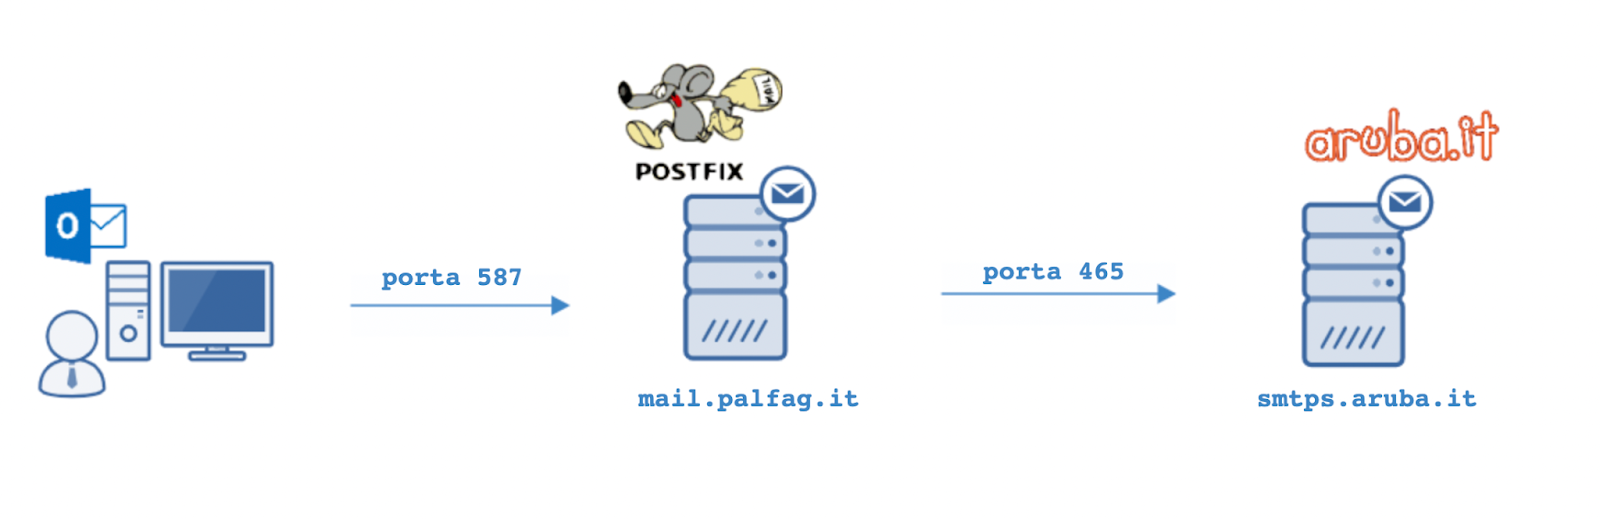
\includegraphics[width=12cm, height=20cm, keepaspectratio]{Screenshot 2021-05-03 at 11.28.07.png}
    \caption{Configurazione di Postfix}\label{confPostfix}
  \end{figure}

1. Innanzitutto sarà necessario installare i seguenti pacchetti:

\begin{verbatim}
    yum install postfix mailx cyrus-sasl cyrus-sasl-plain
\end{verbatim}
2. Creare un file, in questo caso è stato chiamato \textit{sasl\_passwd} dove saranno inserite le credenziali
necessarie per l'autenticazione presso il server Aruba:

\begin{verbatim}
    nano /etc/postfix/sasl_passwd
    [smtps.aruba.it]:465    paolo.fagioli@certimeter.it:pwd
\end{verbatim}
3. Processare il file contenente le credenziali:

\begin{verbatim}
    postmap /etc/postfix/sasl_passwd
\end{verbatim}
4. Editare il file \textit{/etc/postfix/main.cf}:

\begin{verbatim}
    myhostname = mail.palfag.it
    relayhost= [smtps.aruba.it]:465
    mynetworks = 192.168.8.0/24 127.0.0.0/8
    smpd_banner = $myhostname ESMTP $mail_name ($mail_version)
    mailbox_size_limit = 0
    inet_interfaces = all
    inet_protocols = all
    append_dot_mydomain = no
    readme_directory = no
\end{verbatim}
5. Sempre all'interno del file \textit{/etc/postfix/main.cf} inserire i parametri per la configurazione di TLS,
in questo momento saranno necessari il certificato e la chiave precedentemente generati:

\begin{verbatim}
    # TLS parameters
    smtpd_tls_cert_file=/etc/pki/tls/certs/apache-selfsigned.crt
    smtpd_tls_key_file=/etc/pki/tls/private/apache-selfsigned.key

    smtpd_tls_security_level=encrypt
    smtp_tls_CApath=/etc/ssl/certs
    smtp_tls_security_level=encrypt
    smtp_tls_session_cache_database = btree:${data_directory}/smtp_scache
    smtp_sasl_password_maps = hash:/etc/postfix/sasl_passwd
    smtp_tls_wrappermode = yes
    smtp_use_tls = yes
    smtp_sasl_auth_enable = yes
    smtp_sasl_security_options = noanonymous
\end{verbatim}
6. Avviare Postfix:
\begin{verbatim}
    systemctl start postfix.service
\end{verbatim}
7. A questo punto sarà possibile verificare il corretto funzionamento della funzione di inoltro verso i server di Aruba 
provando ad inviare una email da terminale:

\begin{verbatim}
    echo corpo | mail -s “Oggetto” -r emailMittente emailDestinatario 
\end{verbatim}
8. Una volta testato il funzionamento, sarà necessario configurare Postfix in modo che ascolti dalle porte 465 e 587 
(la porta 25 è già configurata di default).

Editare il file \textit{/etc/postfix/master.cf}. Attraverso la seguente configurazione Postfix ascolterà 
sulla porta 587 e sarà dotato di tutte le impostazioni necessarie per supportare il protocollo TLS:

\begin{verbatim}
    submission inet n       -       n       -       -       smtpd
  -o syslog_name=postfix/submission
  -o smtpd_sasl_auth_enable=yes
  -o smtpd_sasl_security_options=noanonymous
  -o broken_sasl_auth_clients=yes
  -o smtpd_tls_security_level=encrypt
  -o smtpd_tls_key_file=/etc/pki/tls/private/apache-selfsigned.key
  -o smtpd_tls_cert_file=/etc/pki/tls/certs/apache-selfsigned.crt
  -o smtpd_tls_loglevel=1
  -o smtpd_tls_session_cache_timeout=3600s
  -o smtpd_tls_session_cache_database=btree:/var/lib/postfix/smtpd_tls_cache
  -o tls_random_source=dev:/dev/urandom
  -o tls_random_exchange_name=/var/lib/postfix/prng_exch
  -o smtpd_tls_auth_only=yes
  -o smtpd_recipient_restrictions=permit_sasl_authenticated,reject
  -o smtpd_relay_restrictions=permit_sasl_authenticated,reject
\end{verbatim}
9. Un procedimento simile per fare in modo che ascolti anche dalla porta 465:

\begin{verbatim}
    smtps     inet  n       -       n       -       -       smtpd
    -o syslog_name=postfix/smtps
    -o smtpd_sasl_auth_enable=yes
    -o smtpd_sasl_security_options=noanonymous
    -o broken_sasl_auth_clients=yes
    -o smtpd_recipient_restrictions=permit_sasl_authenticated,reject
    -o smtpd_tls_security_level=encryptà
    -o smtpd_tls_wrappermode=yes
    -o smtpd_tls_key_file=/etc/pki/tls/private/apache-selfsigned.key
    -o smtpd_tls_cert_file=/etc/pki/tls/certs/apache-selfsigned.crt
    -o smtpd_tls_loglevel=1
    -o smtpd_tls_session_cache_timeout=3600s
    -o smtpd_tls_session_cache_database=btree:/var/lib/postfix/smtpd_tls_cache
    -o tls_random_source=dev:/dev/urandom
    -o tls_random_exchange_name=/var/lib/postfix/prng_exch
    -o smtpd_tls_auth_only=yes
\end{verbatim}
10. Avviare sasl\_authd
\begin{verbatim}
    systemctl start sasl_authd.services
\end{verbatim}
11. Riavviare Postfix
\begin{verbatim}
    systemctl restart postfix.service
\end{verbatim}

Da questo momento Postfix è pronto per svolgere il suo lavoro.

\section{Configurazione Microsoft Outlook}
Il client di posta elettronica standard utilizzato in azienda è Microsoft Outlook, 
per questo motivo la configurazione avverrà con quest'ultimo, 
ma ovviamente il procedimento è analogo utilizzando client mail diversi come ad esempio Mozilla Thunderbird.
Per configurare il client di posta MS Outlook è necessario avviare il software.
A questo punto andare su ``File'' e fare click su ``Aggiungi account''.

Nella finestra proposta inserire il proprio indirizzo di posta aziendale e selezionare ``Consenti la configurazione
manuale dell'account'' e poi fare click su ``Connetti''.

Nella schermata successiva selezionare la voce ``IMAP'' e compilare i campi come mostrato nella tabella seguente:


\begin{table}[htp]
    \centering
    \begin{tabular}{|l|l|l|}
    \hline
    \rowcolor[HTML]{EFEFEF} 
    \textbf{Posta in arrivo} & imaps.aruba.it & 993  \\ \hline
    \textbf{Posta in uscita} & mail.palfag.it & 5555 \\ \hline
    \end{tabular}%
    \end{table}

    Si ricorda che la porta 5555 inserita è una porta effimera che successivamente verrà tradotta nella porta 587
    dal NAT di VirtualBox.
    Selezionare la spunta ``Usa SSL per connetterti'', a questo punto dovremmo trovarci nella stessa situazione
    della figura \ref{confOutlook}.

        \begin{figure}[htp]
            \centering
            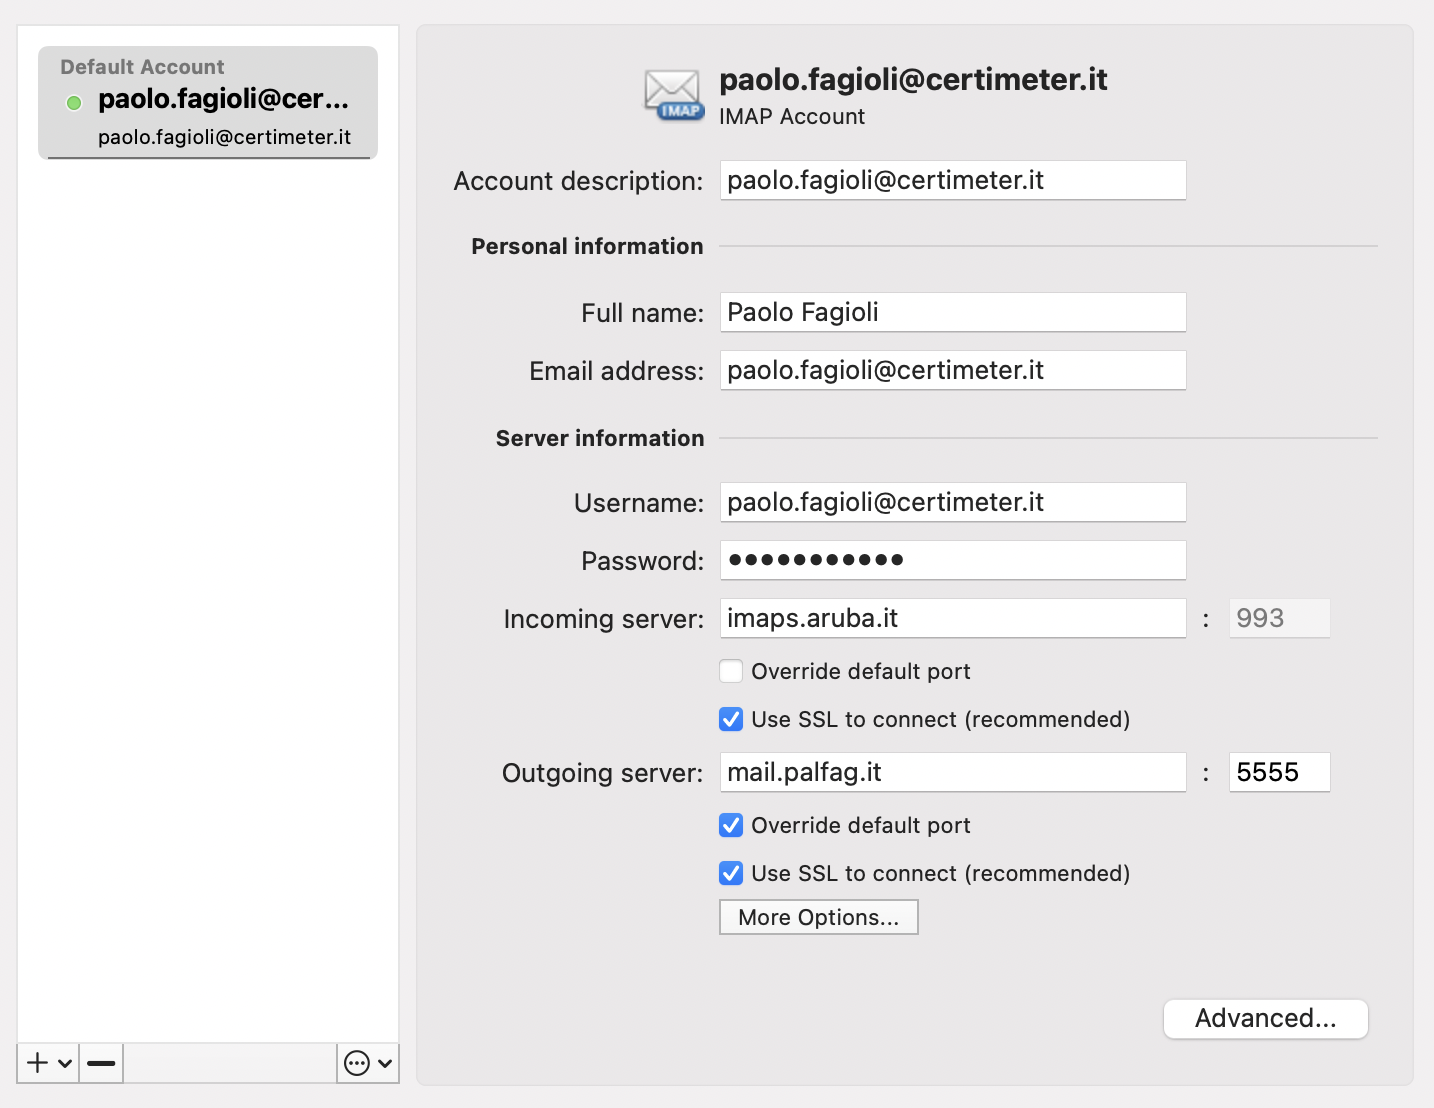
\includegraphics[width=12cm, height=20cm, keepaspectratio]{confOutlook.png}
            \caption{Configurazione di Outlook}\label{confOutlook}
        \end{figure}        
    

    Poiché il dominio mail.palfag.it non è registrato, 
    nessun server DNS sarebbe in grado di compiere la traduzione in 192.168.8.150, 
    sarà dunque necessario inserire un record di traduzione manualmente all’interno del file \textit{/private/etc/hosts} 
    come mostrato nella figura \ref{hosts}.

    \begin{figure}[htp]
        \centering
        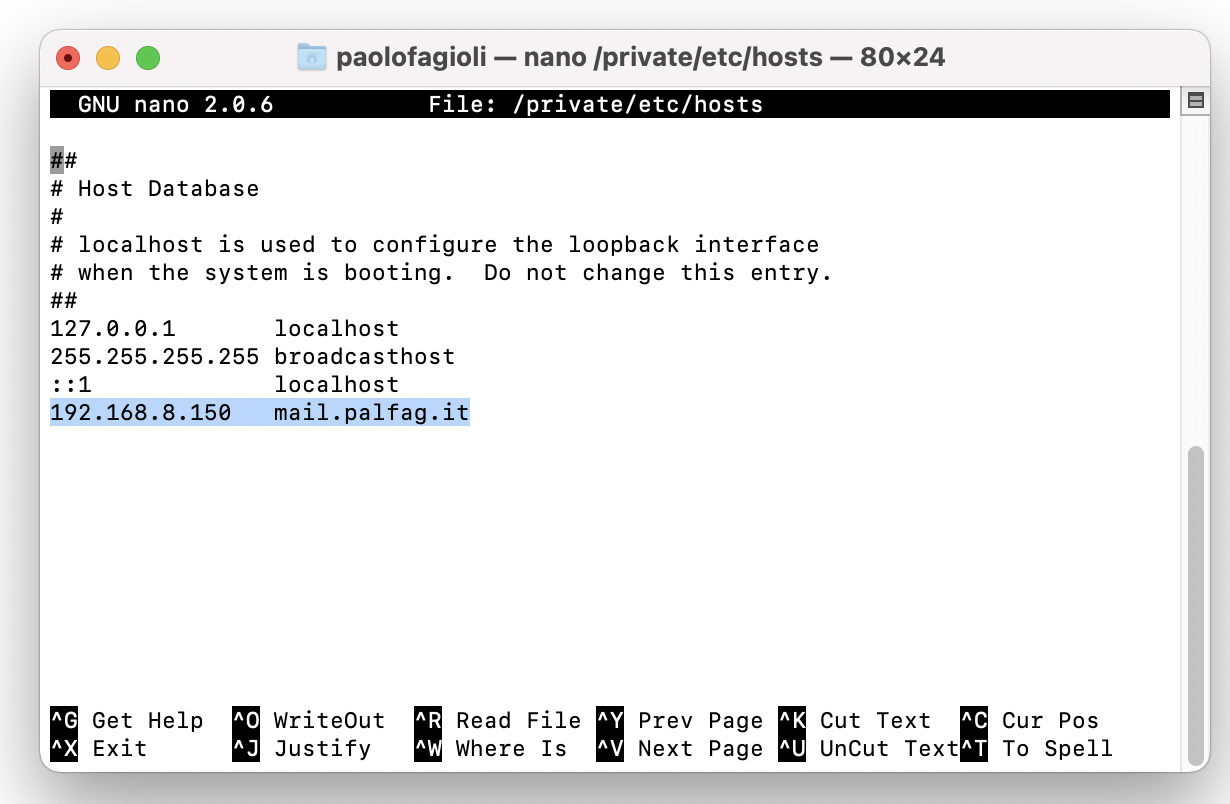
\includegraphics[width=12cm, height=20cm, keepaspectratio]{hosts.png}
        \caption{Aggiunta record di traduzione DNS.}\label{hosts}
    \end{figure}  

    In realtà in azienda ci sarà un server DNS con il compito di tradurre il dominio in indirizzo IP, 
    e non sarebbe più necessario modificare il file \textit{/private/etc/hosts} su ogni macchina aziendale.


    A questo punto è già possibile testare il funzionamento provando ad inviare una email attraverso Outlook. 
    Dovrebbe spuntare un avviso dicendo che il certificato è autofirmato e quindi non attendibile. 
    Sarà necessario istruire il nostro computer a fidarsi sempre del certificato
    (anche in questo caso in azienda non ci sarebbe bisogno di effettuare questo passaggio, poiché 
    il certificato non sarebbe autofirmato, ma firmato da una certificate authority).

    Una volta fatto questo, sarà possibile inviare le email da Outlook.


    \section{Architettura finale}
    Una volta effettuate tutte le configurazioni necessarie, sarà possibile migliorare il disegno dell’architettura. 
    Questo disegno rappresenta una versione più realistica del modello reale, rispetto alla precedente versione.

    \begin{figure}[htp]
        \centering
        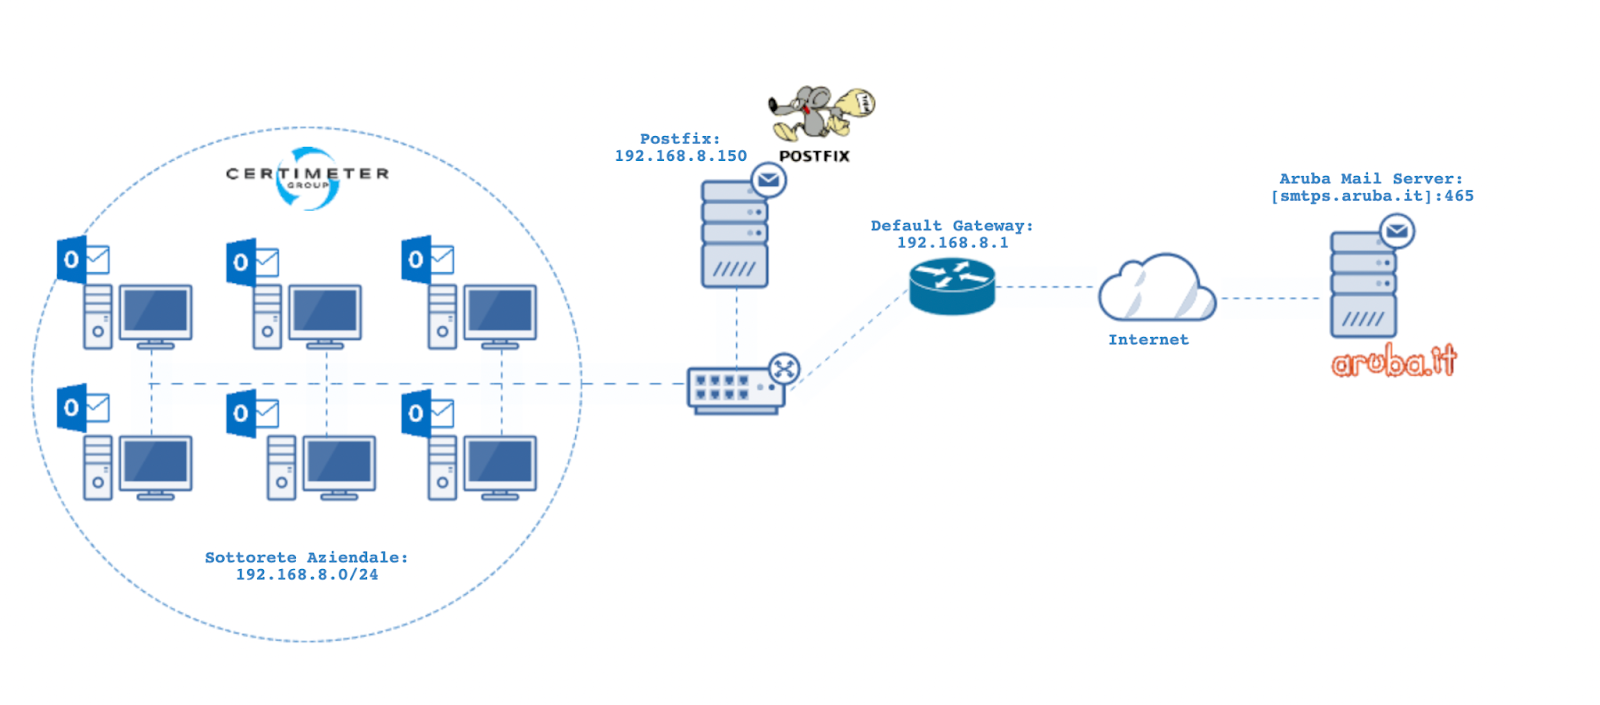
\includegraphics[width=12cm, height=20cm, keepaspectratio]{arch_final.png}
        \caption{Aggiunta record di traduzione DNS.}\label{hosts}
    \end{figure} 

    Tutti i Mail User Agent sono configurati in modo da avere come server SMTP di uscita mail.palfag.it, 
    per la traduzione del dominio, ogni host della rete contatterà il server DNS aziendale, il cui compito è
    quello di risolvere il dominio mail.palfag.it -> 192.168.8.150.

    All'invio di una email da parte di un dipendente, questa verrà indirizzata a Postfix (192.168.8.150) che la 
    ispezionerà. Nel caso in cui dovesse bloccare l’invio della email per via del contenuto sensibile, 
    Postfix provvederà ad avvisare il MUA (nel nostro caso Outlook) del suo rifiuto di consegnare il messaggio.

    Nel caso in cui il messaggio sia autorizzato ad essere inoltrato, Postfix attiverà la sua funzione di inoltro 
    girandolo verso i server mail di Aruba. Fisicamente consegnerà il frame al suo default gateway.

    \pagebreak
    \section{Configurazione di controlli interni}
    Per lo sviluppo di filtri sarà necessario come prima cosa, se non esistono già, creare i file:

    \begin{itemize}
        \item header\_checks
        \item mime\_header\_checks
        \item body\_checks
    \end{itemize}

    All'interno del file header\_checks verranno sviluppati dei controlli per il filtraggio degli header
    (From:, To:, Subject:, ecc\dots), body\_checks si occuperà di effettuare filtri sul corpo del messaggio e
    infine mime\_header\_checks si occuperà degli allegati. È importante notare che il controllo degli allegati
    nativo in Postfix permette soltanto di filtrare in base al nome del file e all'estensione. Successivamente 
    verrà sviluppato un filtro esterno più completo per l'analisi del contenuto degli allegati.

    Una volta creati i file, sarà necessario aggiungere al file \textit{/etc/postfix/main.cf} le seguenti tre righe:

    \begin{verbatim}
        header_checks = regexp:/etc/postfix/header_checks
        mime_header_checks = regexp:/etc/postfix/mime_header_checks
        body_checks = regexp:/etc/postfix/body_checks
    \end{verbatim}

    Postfix utilizzerà questi file per effettuare il filtraggio dei contenuti (es. corpo e oggetto) e anche del
    contesto (es. mittente e destinatario). Sono definiti più file perché Postfix permette di utilizzare regole 
    diverse per filtrare ad esempio oggetto e corpo del messaggio.

    \section{Sviluppo di filtri interni}
    In questo capitolo si provvederà allo sviluppo di una serie di filtri per fare in modo che Postfix possa 
    rilevare eventuali email da bloccare così da prevenire eventuali perdite di dati. 
    Saranno utilizzate le espressioni regolari per lo sviluppo dei filtri. Per ogni filtro sviluppato è possibile 
    decidere in che modo si vuole che reagisca Postfix al verificarsi dell’evento, 
    ovvero quando rileva in un’ email un contenuto identificato sensibile, oppure quando riceve un’email da un 
    mittente inserito in una blacklist.
    I controlli hanno la seguente struttura: “se questo, allora quello”, 
    infatti nella prima parte verrà inserito il pattern del contenuto da rilevare e nella seconda verrà 
    specificata l’azione di risposta da intraprendere.

    Si divideranno i filtri da sviluppare in due macro-aree:

    \begin{enumerate}
        \item Analisi del contenuto;
        \item Analisi del contesto.
    \end{enumerate}

    \subsection{Analisi del contenuto}
    Questo tipo di controlli si occuperà del filtraggio del contenuto dell'email, 
    andando a ispezionare oggetto, corpo del messaggio ed eventuali allegati. 
    
    Saranno utilizzate le espressioni regolari per individuare e bloccare messaggi di posta che contengono dati
    finanziari (ad esempio Carte VISA), o permetterne l’invio eliminando il contenuto sensibile. 
    
    Importante ricordare che Postfix effettua il controllo riga per riga, quindi se viene identificato un 
    contenuto sensibile, e come azione di risposta si scegliesse IGNORE, 
    l’intera riga sarà eliminata (questo potrebbe compromettere l’integrità/significato originale del messaggio). 
    
    Saranno inseriti dei controlli sull’oggetto inserendo parole chiave che, se presenti, 
    potranno portare al blocco dell’invio o alla quarantena del messaggio. Per gli allegati invece è possibile, nativamente,
    effettuare controlli esclusivamente sul filename o sull’estensione. 

    \subsubsection{Controlli sull'oggetto (file header\_checks):}

    1. Blocco delle email che contengono le parole chiave: URGENTE, TOP SECRET, SENSIBILE, SEGRETO.
    In questo caso Postfix bloccherà il messaggio e avviserà il mittente della decisione intrapresa.

    \begin{verbatim}
    /^Subject:(.)*(URGENTE | TOP SECRET| … | SEGRETO)(.)*/
        REJECT Il server ha bloccato il messaggio per 
        la possibile presenza di dati sensibili
    \end{verbatim}
    2. Quarantena dei messaggi che contengono la parola chiave PRIVATO:
    \begin{verbatim}
    /^Subject:(.)*PRIVATO(.)*/
        HOLD Il server ha messo in quarantena il messaggio per 
        la possibile presenza di dati sensibili
    \end{verbatim}
    3. Blocco dei messaggi che hanno come oggetto una carta VISA:
    \begin{verbatim}
    /^Subject:(.)*([0-9]{4}( |-)*){3}[0-9]{4}(.)*/
        REJECT EMAIL BLOCCATA: CARTA VISA RICONOSCIUTA
    \end{verbatim}


    \subsubsection{Controlli sull'allegato (file mime\_header\_checks):}

    1. Blocco delle email che contengono allegati con estensione .ZIP:

    \begin{verbatim}
    /^(.)*name=\"(.*)\.zip\"/
        REJECT allegato ZIP Bloccato
    \end{verbatim}

    \subsubsection{Controlli sul corpo (file body\_checks):}

    1. Blocco carte VISA presenti nel corpo del messaggio:
    \begin{verbatim}
    /^(.)*([0-9]{4}( |-)*){3}[0-9]{4}(.)*/
        REJECT EMAIL BLOCCATA: CARTA VISA RICONOSCIUTA
    \end{verbatim}
    2. Eliminazione del codice fiscale presente nel messaggio:
    \begin{verbatim}
    /^(.)*([A-z]){6}([0-9]){2}[A-z]([0-9]){2}[A-z][0-9]{3}[A-z](.)*/
        IGNORE CODICE FISCALE RIMOSSO DAL MESSAGGIO
    \end{verbatim}


    \subsection{Analisi del contesto}
    In quest’area i controlli tratteranno il contesto e quindi andranno a focalizzarsi sulle restanti 
    informazioni che compongono l’email. Saranno creati, ad esempio, controlli per filtrare in base al 
    mittente del messaggio o del destinatario. 
    Verrà bloccato l’invio delle email aziendali per un preciso dominio e si potrà decidere che Postfix 
    non accetti email che provengono da un account di posta elettronica diverso da quello aziendale 
    (nome.cognome@certimeter.it). 

    \subsubsection{Mettere in blacklist un mittente:}
    Come impostazione di default Postfix accetta le email che provengono da qualunque indirizzo di posta, 
    tuttavia è possibile inserire un mittente in blacklist in modo che postfix rifiuti tutte le email che 
    provengono dal suo indirizzo di posta. Vi sono diverse possibilità per mettere un mittente in blacklist, 
    tuttavia tutte effettuano un controllo sull’header FROM: del messaggio.

    \begin{verbatim}
    /^From:(.)*francesco.lorusso@certimeter.it(.)*/
        REJECT  SENDER ADDRESS REJECTED: BLACKLISTED
    \end{verbatim}

    \subsubsection{Blocco delle email indirizzate ad un certo dominio:}
    Si può supporre ad esempio che da policy aziendali sia vietato, per i dipendenti, 
    inviare email al dominio reply.it.
    In questo caso verrà inserito il seguente filtro:

    \begin{verbatim}
    /^To:.*@reply.it/
        REJECT RECIPIENT DOMAIN BANNED
    \end{verbatim}

    \subsubsection{Blocco delle email inviate da caselle di posta differenti da quelle aziendali:}
    \begin{verbatim}
    if /^From:/
    !/(^From:.*@certimeter.it)/ 
        REJECT SENDER NON-CORPORATE DOMAIN REJECTED
    endif
    \end{verbatim}

    \section{Script Python esterno per la gestione degli allegati}
    Il filtraggio dei contenuti di Postfix è abbastanza limitato, poiché non permette di analizzare il contenuto
    degli allegati. Postfix però prevede la possibilità di utilizzare dei plug-in esterni. Per questo motivo è stato
    sviluppato uno script Python che permettesse l'analisi e l'identificazione di contenuti sensibili presenti 
    negli allegati.


    \section{Shell code}
    Nel suo sito ufficiale Postfix offre uno script bash di esempio che è possibile personalizzare per  
    permettere il dialogo tra il mail server Postfix e lo script(Python) sviluppato. Lo script avrà la funzione di mediatore tra Postfix e Python. 
    In ingresso gira la email, che Postfix consegna allo script wrapper.sh, allo script Python 
    il cui compito è quello di analizzarla.
    In base al valore di uscita dello script Python, wrapper.sh si comporterà in due modi:

    
    \begin{enumerate}
        \item se sys.exit(0): ritorna la email a Postfix in modo che possa continuare il percorso;
        \item se sys.exit(1): il messaggio viene rifiutato poiché trovati dati sensibili. (Postfix invierà una 
        email di ritorno al mittente spiegando che non ha dovuto bloccare il messaggio). 
    \end{enumerate}

    \begin{verbatim}
1 #!/bin/sh
2 
3 # Simple shell-based filter. It is meant to be invoked as follows:
4 #       /path/to/script -f sender recipients...
5 
6 # Localize these. The -G option does nothing before Postfix 2.3.
7 INSPECT_DIR=/var/spool/filter
8 SENDMAIL="/usr/sbin/sendmail -G -i" # NEVER NEVER NEVER use "-t" here.
9 
10 # Exit codes from <sysexits.h>
11 EX_TEMPFAIL=75
12 EX_UNAVAILABLE=69
13 
14 # Clean up when done or when aborting.
15 trap "rm -f in.$$" 0 1 2 3 15
16 
17 # Start processing.
18 cd $INSPECT_DIR || {
19     echo $INSPECT_DIR does not exist; exit $EX_TEMPFAIL; }
20 
21 cat >in.$$ || { 
22     echo Cannot save mail to file; exit $EX_TEMPFAIL; }
23 
24 # Specify your content filter here.
25 # python3 /media/shared/my_filter.py <in.$$ || {
26 #   echo Message content rejected; exit $EX_UNAVAILABLE; }
27 
28 $SENDMAIL "$@" <in.$$
29 
30 exit $?
    \end{verbatim}

    \section{Integrazione script esterno}
    Per fare in modo che venga eseguito il filtro esterno, sarà necessario configurare Postfix in modo
    che consegni l'email allo script.
    
    1. Prima di tutto sarà necessario aggiungere nel file \textit{/etc/postfix/master.cf} il filtro:

    \begin{verbatim}
    /etc/postfix/master.cf:
    # =============================================================
    # service type  private unpriv  chroot  wakeup  maxproc command
    #               (yes)   (yes)   (yes)   (never) (100)
    # =============================================================
    my_filter unix	  -	      n	      n	      -	      -	    pipe
	    flags=Rq user=filter 
        argv=/home/filter/wrapper.sh -f ${sender} -- ${recipient}
    \end{verbatim}
    In questo modo è stato registrato il filtro chiamato ``my\_filter''.
    
    2. Adesso bisogna istruire Postfix di eseguire lo script quando riceve le email sulla porta 587 (submission):

    \begin{verbatim}
        /etc/postfix/master.cf:
    # =============================================================
    # service type  private unpriv  chroot  wakeup  maxproc command
    #               (yes)   (yes)   (yes)   (never) (100)
    # =============================================================
    submission inet   n       -       n        -      -      smtpd
            -o content_filter=my_filter:  
    \end{verbatim}
    
    3. Infine sarà necessario riavviare postfix:

    \begin{verbatim}
    postfix reload 
    \end{verbatim}
    

    \section{Test}
    In questo paragrafo verranno effettuati una serie di test volti a collaudare la soluzione DLP 
    implementata e a verificarne il corretto funzionamento.

    \subsection{Test sull'analisi del contenuto}


\begin{table}[htp]
    \centering
    \resizebox{\textwidth}{!}{%
    \begin{tabular}{ll}
    \multicolumn{2}{c}{test 1 (TS01): \textbf{Messaggio contenente parola chiave da bloccare}}                                                              \\ \hline
    \rowcolor[HTML]{EFEFEF} 
    \multicolumn{1}{|l|}{\cellcolor[HTML]{EFEFEF}ID}    & \multicolumn{1}{l|}{\cellcolor[HTML]{EFEFEF}TS01}                            \\ \hline
    \multicolumn{1}{|l|}{Nome}                          & \multicolumn{1}{l|}{Messaggio contenente parola chiave}                      \\ \hline
    \rowcolor[HTML]{EFEFEF} 
    \multicolumn{1}{|l|}{\cellcolor[HTML]{EFEFEF}Descrizione} &
      \multicolumn{1}{l|}{\cellcolor[HTML]{EFEFEF}\begin{tabular}[c]{@{}l@{}}il messaggio inviato contiene la parola chiave \\ TOP SECRET come oggetto del messaggio\end{tabular}} \\ \hline
    \multicolumn{1}{|l|}{\begin{tabular}[c]{@{}l@{}}Messaggio inviato\\ dal mittente\end{tabular}} &
      \multicolumn{1}{l|}{\begin{tabular}[c]{@{}l@{}}Subject: Top secret\\ From: Paolo Fagioli <paolo.fagioli@certimeter.it>\\ To: Paolo Fagioli <palfag33@gmail.com>\\ \\ Test TS01\end{tabular}} \\ \hline
    \rowcolor[HTML]{EFEFEF} 
    \multicolumn{1}{|l|}{\cellcolor[HTML]{EFEFEF}Risultato atteso} &
      \multicolumn{1}{l|}{\cellcolor[HTML]{EFEFEF}\begin{tabular}[c]{@{}l@{}}Verrà attivata la clausola REJECT, il messaggio\\ sarà rifiutato da Postfix e verrà avvisato il \\ mittente.\end{tabular}} \\ \hline
    \multicolumn{1}{|l|}{Risultato ottenuto} &
      \multicolumn{1}{l|}{\begin{tabular}[c]{@{}l@{}}Postfix ha rifiutato il messaggio. Il mittente ha \\ ricevuto il seguente avviso:\\ \\ Il server ha bloccato il messaggio per\\ la possibile presenza di dati sensibili.\end{tabular}} \\ \hline
    \rowcolor[HTML]{EFEFEF} 
    \multicolumn{1}{|l|}{\cellcolor[HTML]{EFEFEF}Esito} & \multicolumn{1}{l|}{\cellcolor[HTML]{EFEFEF}{\color[HTML]{333333} SUPERATO}} \\ \hline
    \end{tabular}%
    }
    \end{table}


\begin{table}[htp]
    \centering
    \resizebox{\textwidth}{!}{%
    \begin{tabular}{ll}
    \multicolumn{2}{c}{test 2 (TS02): \textbf{Messaggio privo di dati sensibili}} \\ \hline
    \rowcolor[HTML]{EFEFEF} 
    \multicolumn{1}{|l|}{\cellcolor[HTML]{EFEFEF}ID} &
      \multicolumn{1}{l|}{\cellcolor[HTML]{EFEFEF}TS02} \\ \hline
    \multicolumn{1}{|l|}{Nome} &
      \multicolumn{1}{l|}{Messaggio privo di dati sensibili} \\ \hline
    \rowcolor[HTML]{EFEFEF} 
    \multicolumn{1}{|l|}{\cellcolor[HTML]{EFEFEF}Descrizione} &
      \multicolumn{1}{l|}{\cellcolor[HTML]{EFEFEF}\begin{tabular}[c]{@{}l@{}}il messaggio inviato non contiene alcun dato\\ sensibile\end{tabular}} \\ \hline
    \multicolumn{1}{|l|}{\begin{tabular}[c]{@{}l@{}}Messaggio inviato\\ dal mittente\end{tabular}} &
      \multicolumn{1}{l|}{\begin{tabular}[c]{@{}l@{}}Subject: Benvenuto!\\ From: Paolo Fagioli <paolo.fagioli@certimeter.it>\\ To: Paolo Fagioli <palfag33@gmail.com>\\ \\ \\ Ciao Paolo,\\ Benvenuto nel Team <3\end{tabular}} \\ \hline
    \rowcolor[HTML]{EFEFEF} 
    \multicolumn{1}{|l|}{\cellcolor[HTML]{EFEFEF}Risultato atteso} &
      \multicolumn{1}{l|}{\cellcolor[HTML]{EFEFEF}\begin{tabular}[c]{@{}l@{}}In questo caso Postfix si comporterà da normale\\ mail server di inoltro. Il messaggio verrà \\ inoltrato presso i mail server di Aruba.\end{tabular}} \\ \hline
    \multicolumn{1}{|l|}{Risultato ottenuto} &
      \multicolumn{1}{l|}{\begin{tabular}[c]{@{}l@{}}Come da previsione il messaggio è stato\\ inoltrato correttamente. Il destinatario ha \\ ricevuto il seguente messaggio:\\ \\ Subject: Benvenuto!\\ From: Paolo Fagioli <paolo.fagioli@certimeter.it>\\ To: Paolo Fagioli <palfag33@gmail.com>\\ \\ Ciao Paolo,\\ Benvenuto nel Team <3\end{tabular}} \\ \hline
    \rowcolor[HTML]{EFEFEF} 
    \multicolumn{1}{|l|}{\cellcolor[HTML]{EFEFEF}Esito} &
      \multicolumn{1}{l|}{\cellcolor[HTML]{EFEFEF}{\color[HTML]{333333} SUPERATO}} \\ \hline
    \end{tabular}%
    }
    \end{table}

\begin{table}[htp]
    \centering
    \resizebox{\textwidth}{!}{%
    \begin{tabular}{ll}
    \multicolumn{2}{c}{test 3 (TS03): \textbf{Messaggio contenente dati personali}}                                                                                   \\ \hline
    \rowcolor[HTML]{EFEFEF} 
    \multicolumn{1}{|l|}{\cellcolor[HTML]{EFEFEF}ID}          & \multicolumn{1}{l|}{\cellcolor[HTML]{EFEFEF}TS03}                                            \\ \hline
    \multicolumn{1}{|l|}{Nome}                                & \multicolumn{1}{l|}{Messaggio contenente dati personali}                                     \\ \hline
    \rowcolor[HTML]{EFEFEF} 
    \multicolumn{1}{|l|}{\cellcolor[HTML]{EFEFEF}Descrizione} & \multicolumn{1}{l|}{\cellcolor[HTML]{EFEFEF}il messaggio inviato contiene un codice fiscale} \\ \hline
    \multicolumn{1}{|l|}{\begin{tabular}[c]{@{}l@{}}Messaggio inviato\\ dal mittente\end{tabular}} &
      \multicolumn{1}{l|}{\begin{tabular}[c]{@{}l@{}}Subject: Aggiornamento\\ From: Paolo Fagioli <paolo.fagioli@certimeter.it>\\ To: Paolo Fagioli <palfag33@gmail.com>\\ \\ Salve invio quanto richiesto,\\ Nominativo:\\ 	Paolo Fagioli\\ Codice fiscale:\\ 	TCMDPW34L46D127O\\ Buona giornata,\\ Paolo\end{tabular}} \\ \hline
    \rowcolor[HTML]{EFEFEF} 
    \multicolumn{1}{|l|}{\cellcolor[HTML]{EFEFEF}Risultato atteso} &
      \multicolumn{1}{l|}{\cellcolor[HTML]{EFEFEF}\begin{tabular}[c]{@{}l@{}}Verrà attivata la clausola IGNORE, il codice\\ fiscale sarà rimosso e la restante parte del\\ messaggio verrà ricevuta dal destinatario.\end{tabular}} \\ \hline
    \multicolumn{1}{|l|}{Risultato ottenuto} &
      \multicolumn{1}{l|}{\begin{tabular}[c]{@{}l@{}}Postfix si è comportato come previsto, eliminando\\ il codice fiscale dal messaggio. Il messaggio\\ ricevuto dal destinatario è il seguente:\\ \\ Salve invio quanto richiesto,\\ Nominativo:\\         Paolo Fagioli\\ Codice fiscale:\\ \\ Buona giornata,\\ Paolo\end{tabular}} \\ \hline
    \rowcolor[HTML]{EFEFEF} 
    \multicolumn{1}{|l|}{\cellcolor[HTML]{EFEFEF}Esito}       & \multicolumn{1}{l|}{\cellcolor[HTML]{EFEFEF}SUPERATO}                                        \\ \hline
    \end{tabular}%
    }
    \end{table}


\begin{table}[htp]
    \centering
    \resizebox{\textwidth}{!}{%
    \begin{tabular}{ll}
    \multicolumn{2}{c}{test 4 (TS04): \textbf{Messaggio contenente dati finanziari}} \\ \hline
    \rowcolor[HTML]{EFEFEF} 
    \multicolumn{1}{|l|}{\cellcolor[HTML]{EFEFEF}ID} &
      \multicolumn{1}{l|}{\cellcolor[HTML]{EFEFEF}TS04} \\ \hline
    \multicolumn{1}{|l|}{Nome} &
      \multicolumn{1}{l|}{Messaggio contenente dati finanziari} \\ \hline
    \rowcolor[HTML]{EFEFEF} 
    \multicolumn{1}{|l|}{\cellcolor[HTML]{EFEFEF}Descrizione} &
      \multicolumn{1}{l|}{\cellcolor[HTML]{EFEFEF}\begin{tabular}[c]{@{}l@{}}il messaggio inviato contiene il numero di una\\ carta di pagamento VISA\end{tabular}} \\ \hline
    \multicolumn{1}{|l|}{\begin{tabular}[c]{@{}l@{}}Messaggio inviato\\ dal mittente\end{tabular}} &
      \multicolumn{1}{l|}{\begin{tabular}[c]{@{}l@{}}Subject: pagamento\\ From: Paolo Fagioli <paolo.fagioli@certimeter.it>\\ To: Paolo Fagioli <palfag33@gmail.com>\\ \\ Ciao,\\ ti invio il numero della carta:\\ 4839-9268-2312-5203\\ Mi raccomando usala solo per urgenze.\\ Paolo\end{tabular}} \\ \hline
    \rowcolor[HTML]{EFEFEF} 
    \multicolumn{1}{|l|}{\cellcolor[HTML]{EFEFEF}Risultato atteso} &
      \multicolumn{1}{l|}{\cellcolor[HTML]{EFEFEF}\begin{tabular}[c]{@{}l@{}}Verrà attivata la clausola REJECT, il messaggio\\ sarà rifiutato da Postfix e verrà avvisato il\\ mittente.\end{tabular}} \\ \hline
    \multicolumn{1}{|l|}{Risultato ottenuto} &
      \multicolumn{1}{l|}{\begin{tabular}[c]{@{}l@{}}Postfix ha rifiutato il messaggio. Il mittente ha\\ ricevuto il seguente avviso:\\ \\ EMAIL BLOCCATA: \\ CARTA VISA RICONOSCIUTA\end{tabular}} \\ \hline
    \rowcolor[HTML]{EFEFEF} 
    \multicolumn{1}{|l|}{\cellcolor[HTML]{EFEFEF}Esito} &
      \multicolumn{1}{l|}{\cellcolor[HTML]{EFEFEF}{\color[HTML]{333333} SUPERATO}} \\ \hline
    \end{tabular}%
    }
    \end{table}

    \pagebreak

\begin{table}[htp]
    \centering
    \resizebox{\textwidth}{!}{%
    \begin{tabular}{ll}
    \multicolumn{2}{c}{test 5 (TS05): \textbf{Messaggio contenente allegato sensibile}}                                                         \\ \hline
    \rowcolor[HTML]{EFEFEF} 
    \multicolumn{1}{|l|}{\cellcolor[HTML]{EFEFEF}ID}    & \multicolumn{1}{l|}{\cellcolor[HTML]{EFEFEF}TS05}                            \\ \hline
    \multicolumn{1}{|l|}{Nome}                          & \multicolumn{1}{l|}{Messaggio contenente allegato sensibile}                 \\ \hline
    \rowcolor[HTML]{EFEFEF} 
    \multicolumn{1}{|l|}{\cellcolor[HTML]{EFEFEF}Descrizione} &
      \multicolumn{1}{l|}{\cellcolor[HTML]{EFEFEF}\begin{tabular}[c]{@{}l@{}}il messaggio inviato contiene come allegato.\end{tabular}} \\ \hline
    \multicolumn{1}{|l|}{\begin{tabular}[c]{@{}l@{}}Messaggio inviato\\ dal mittente\end{tabular}} &
      \multicolumn{1}{l|}{\begin{tabular}[c]{@{}l@{}}Subject: test\\ From: Paolo Fagioli <paolo.fagioli@certimeter.it>\\ To: Paolo Fagioli <palfag33@gmail.com>\\ \\ test con allegato.\end{tabular}} \\ \hline
    \rowcolor[HTML]{EFEFEF} 
    \multicolumn{1}{|l|}{\cellcolor[HTML]{EFEFEF}Risultato atteso} &
      \multicolumn{1}{l|}{\cellcolor[HTML]{EFEFEF}\begin{tabular}[c]{@{}l@{}}Il filtro nativo di Postfix non troverà nulla, passerà\\ il messaggio al filtro esterno sviluppato in Python.\\ Il filtro esterno troverà il contenuto sensibile e \\ bloccherà l'invio, e verrà inviata una email di \\ rimbalzo al mittente.\end{tabular}} \\ \hline
    \multicolumn{1}{|l|}{Risultato ottenuto} &
      \multicolumn{1}{l|}{\begin{tabular}[c]{@{}l@{}}Il risultato ottenuto conferma le aspettative.\\ Il mittente riceve la seguente email:\\ \\ Subject: Undelivered Mail Returned to Sender\\ From: Mail Delivery System <MAILER-DAEMON@mail.palfag.it>\\ To: Paolo Fagioli <paolo.fagioli@certimeter.it>\\ \\ Message content rejected\end{tabular}} \\ \hline
    \rowcolor[HTML]{EFEFEF} 
    \multicolumn{1}{|l|}{\cellcolor[HTML]{EFEFEF}Esito} & \multicolumn{1}{l|}{\cellcolor[HTML]{EFEFEF}{\color[HTML]{333333} SUPERATO}} \\ \hline
    \end{tabular}%
    }
    \end{table}

    \begin{figure}[!b]
        \centering
        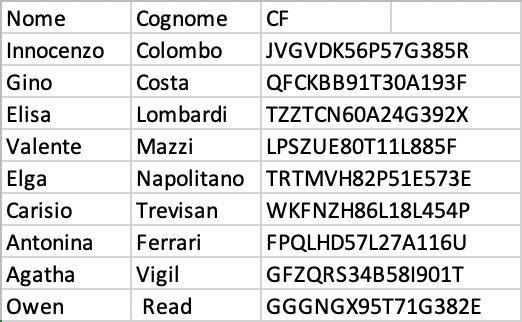
\includegraphics[width=8cm, height=10cm, keepaspectratio]{allegato_excel.png}
        \caption{Allegato elenco\_dipendenti.csv}\label{allegatoExcel}
      \end{figure}

    

    %\pagebreak

\begin{table}[htp]
    \centering
    \resizebox{\textwidth}{!}{%
    \begin{tabular}{ll}
    \multicolumn{2}{c}{test 6 (TS06): \textbf{Messaggio contenente allegato innocuo}} \\ \hline
    \rowcolor[HTML]{EFEFEF} 
    \multicolumn{1}{|l|}{\cellcolor[HTML]{EFEFEF}ID} &
      \multicolumn{1}{l|}{\cellcolor[HTML]{EFEFEF}TS06} \\ \hline
    \multicolumn{1}{|l|}{Nome} &
      \multicolumn{1}{l|}{Messaggio contenente allegato innocuo} \\ \hline
    \rowcolor[HTML]{EFEFEF} 
    \multicolumn{1}{|l|}{\cellcolor[HTML]{EFEFEF}Descrizione} &
      \multicolumn{1}{l|}{\cellcolor[HTML]{EFEFEF}\begin{tabular}[c]{@{}l@{}}il messaggio inviato contiene come allegato\\ un file word non contenente dati sensibili.\\ \\ allegato: poesia.doc\end{tabular}} \\ \hline
    \multicolumn{1}{|l|}{\begin{tabular}[c]{@{}l@{}}Messaggio inviato\\ dal mittente\end{tabular}} &
      \multicolumn{1}{l|}{\begin{tabular}[c]{@{}l@{}}Subject: test\\ From: Paolo Fagioli <paolo.fagioli@certimeter.it>\\ To: Paolo Fagioli <palfag33@gmail.com>\\ \\ test con allegato.\end{tabular}} \\ \hline
    \rowcolor[HTML]{EFEFEF} 
    \multicolumn{1}{|l|}{\cellcolor[HTML]{EFEFEF}Risultato atteso} &
      \multicolumn{1}{l|}{\cellcolor[HTML]{EFEFEF}\begin{tabular}[c]{@{}l@{}}Il filtro nativo di Postfix non troverà nulla, passerà\\ il messaggio al filtro esterno sviluppato in Python.\\ Il filtro esterno non troverà alcun contenuto sensibile e \\ restituirà l'email a Postfix tramite il comando sendmail.\\ L'email sarà inoltrata ai mail server di Aruba.\end{tabular}} \\ \hline
    \multicolumn{1}{|l|}{Risultato ottenuto} &
      \multicolumn{1}{l|}{\begin{tabular}[c]{@{}l@{}}Il risultato ottenuto conferma le aspettative.\\ Il mittente ha ricevuto l'email originale contenente il file word.\end{tabular}} \\ \hline
    \rowcolor[HTML]{EFEFEF} 
    \multicolumn{1}{|l|}{\cellcolor[HTML]{EFEFEF}Esito} &
      \multicolumn{1}{l|}{\cellcolor[HTML]{EFEFEF}{\color[HTML]{333333} SUPERATO}} \\ \hline
    \end{tabular}%
    }
    \end{table}

    \begin{figure}[htp]
        \centering
        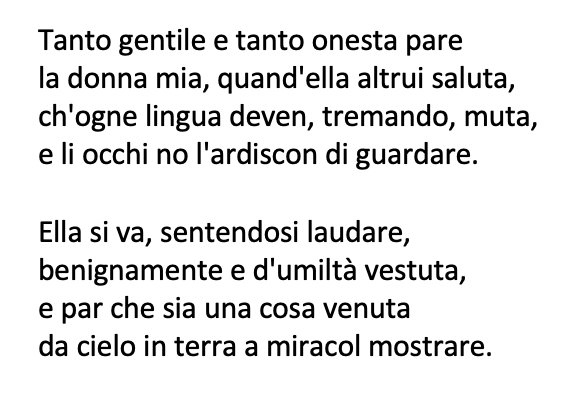
\includegraphics[width=8cm, height=10cm, keepaspectratio]{allegato_word.png}
        \caption{Allegato poesia.doc}\label{allegatoWord}
      \end{figure}



    \pagebreak
    \subsection{Test sull'analisi del contesto}
    


\begin{table}[htp]
    \vspace{4.5cm}
    \centering
    \resizebox{\textwidth}{!}{%
    \begin{tabular}{ll}
    \multicolumn{2}{c}{test 7 (TS07): \textbf{Messaggio indirizzato al dominio reply.it}}                                                       \\ \hline
    \rowcolor[HTML]{EFEFEF} 
    \multicolumn{1}{|l|}{\cellcolor[HTML]{EFEFEF}ID}    & \multicolumn{1}{l|}{\cellcolor[HTML]{EFEFEF}TS07}                            \\ \hline
    \multicolumn{1}{|l|}{Nome}                          & \multicolumn{1}{l|}{Messaggio indirizzato al dominio reply.it}               \\ \hline
    \rowcolor[HTML]{EFEFEF} 
    \multicolumn{1}{|l|}{\cellcolor[HTML]{EFEFEF}Descrizione} &
      \multicolumn{1}{l|}{\cellcolor[HTML]{EFEFEF}\begin{tabular}[c]{@{}l@{}}il messaggio è stato inviato ad un \\ dominio bloccato da policy.\end{tabular}} \\ \hline
    \multicolumn{1}{|l|}{\begin{tabular}[c]{@{}l@{}}Messaggio inviato\\ dal mittente\end{tabular}} &
      \multicolumn{1}{l|}{\begin{tabular}[c]{@{}l@{}}Subject: test invio\\ From: Paolo Fagioli <paolo.fagioli@certimeter.it>\\ To: Paolo Fagioli <p.fagioli@reply.it>\\ \\ prova\end{tabular}} \\ \hline
    \rowcolor[HTML]{EFEFEF} 
    \multicolumn{1}{|l|}{\cellcolor[HTML]{EFEFEF}Risultato atteso} &
      \multicolumn{1}{l|}{\cellcolor[HTML]{EFEFEF}\begin{tabular}[c]{@{}l@{}}Verrà attivata la clausola REJECT, il messaggio\\ sarà rifiutato da Postfix e verrà avvisato il\\ mittente.\end{tabular}} \\ \hline
    \multicolumn{1}{|l|}{Risultato ottenuto} &
      \multicolumn{1}{l|}{\begin{tabular}[c]{@{}l@{}}Postfix ha rifiutato il messaggio. Il mittente ha\\ ricevuto il seguente avviso:\\ \\ RECIPIENT DOMAIN BANNED\end{tabular}} \\ \hline
    \rowcolor[HTML]{EFEFEF} 
    \multicolumn{1}{|l|}{\cellcolor[HTML]{EFEFEF}Esito} & \multicolumn{1}{l|}{\cellcolor[HTML]{EFEFEF}{\color[HTML]{333333} SUPERATO}} \\ \hline
    \end{tabular}%
    }
    \end{table}


\begin{table}[htp]
    \centering
    \resizebox{\textwidth}{!}{%
    \begin{tabular}{ll}
    \multicolumn{2}{c}{test 8 (TS08): \textbf{Messaggio inviato da mittente in blacklist}} \\ \hline
    \rowcolor[HTML]{EFEFEF} 
    \multicolumn{1}{|l|}{\cellcolor[HTML]{EFEFEF}ID} &
      \multicolumn{1}{l|}{\cellcolor[HTML]{EFEFEF}TS08} \\ \hline
    \multicolumn{1}{|l|}{Nome} &
      \multicolumn{1}{l|}{Messaggio inviato da mittente in blacklist} \\ \hline
    \rowcolor[HTML]{EFEFEF} 
    \multicolumn{1}{|l|}{\cellcolor[HTML]{EFEFEF}Descrizione} &
      \multicolumn{1}{l|}{\cellcolor[HTML]{EFEFEF}\begin{tabular}[c]{@{}l@{}}il messaggio è stato inviato da un \\ mittente che si trova in blacklist.\end{tabular}} \\ \hline
    \multicolumn{1}{|l|}{\begin{tabular}[c]{@{}l@{}}Messaggio inviato\\ dal mittente\end{tabular}} &
      \multicolumn{1}{l|}{\begin{tabular}[c]{@{}l@{}}Subject: avviso\\ From: Francesco Lorusso <francesco.lorusso@certimeter.it>\\ To: Paolo Fagioli <paolo.fagioli@certimeter.it>\\ \\ ciao Paolo,\\ ti avviso che domani non sarà possibile vederci.\end{tabular}} \\ \hline
    \rowcolor[HTML]{EFEFEF} 
    \multicolumn{1}{|l|}{\cellcolor[HTML]{EFEFEF}Risultato atteso} &
      \multicolumn{1}{l|}{\cellcolor[HTML]{EFEFEF}\begin{tabular}[c]{@{}l@{}}Verrà attivata la clausola REJECT, il messaggio\\ sarà rifiutato da Postfix e verrà avvisato il\\ mittente.\end{tabular}} \\ \hline
    \multicolumn{1}{|l|}{Risultato ottenuto} &
      \multicolumn{1}{l|}{\begin{tabular}[c]{@{}l@{}}Postfix ha rifiutato il messaggio. Il mittente ha\\ ricevuto il seguente avviso:\\ \\ SENDER ADDRESS REJECTED: BLACKLISTED\end{tabular}} \\ \hline
    \rowcolor[HTML]{EFEFEF} 
    \multicolumn{1}{|l|}{\cellcolor[HTML]{EFEFEF}Esito} &
      \multicolumn{1}{l|}{\cellcolor[HTML]{EFEFEF}{\color[HTML]{333333} SUPERATO}} \\ \hline
    \end{tabular}%
    }
    \end{table}






    \chapter{Conclusioni e sviluppi futuri}

\section{Sviluppi futuri}


    %\appendix

    %\chapter{Script per la gestione degli allegati}

\begin{verbatim}
import sys
import email
import base64
import re
from tika import parser
import os




# REGEX TO CHECK
visa_card_pattern = '^(.|\n)*([0-9]{4}( |-)*){3}[0-9]{4}(.|\n)*'
codice_fiscale_pattern = '(.|\n)*([A-z]){6}([0-9]){2}[A-z]([0-9]\
                        ){2}[A-z][0-9]{3}[A-z](.|\n)*'



filename = sys.stdin.read()


filename2 = "email.eml"
fd = open(filename2, 'w')
fd.write(filename)
#print(fd)
fd.close()



is_sensitive_data_found = False


msg = email.message_from_file(open(filename2))


content_type = msg.get('content-type')
type = content_type.split(';')[0]


#if msg.is_multipart():
if(type == 'multipart/mixed'):
    attachments = msg.get_payload()

    for attachment in attachments:

        if attachment.get_filename() is not None:
           
            filename = attachment.get_filename()
            extension = filename.split(".")[-1]

            if(extension == "txt"):

                payload = attachment.get_payload()

                decoded = base64.b64decode(payload)

                decoded_utf = decoded.decode("utf-8")

                print(decoded_utf)
                result = re.match(visa_card_pattern, decoded_utf) or \
                         re.match(codice_fiscale_pattern, decoded_utf)
                

                if result:
                    is_sensitive_data_found = True
                    break
                else:
                    print("nessun dato sensibile trovato")


            elif (extension == "doc" or
                  extension == "pdf" or
                  extension == "csv" or
                  extension == "ppt"):


                bytes = attachment.get_payload(decode=True)
                

                new_filename = 'file.' + extension
                f = open(new_filename, 'wb')
                f.write(bytes)
                f.close()

                text = parser.from_file(new_filename, 'http://localhost:9998/tika')
                parsed_text = text['content']

                print(parsed_text)

                result = bool(re.match(visa_card_pattern, parsed_text) or\
                              re.match(codice_fiscale_pattern, parsed_text))

                os.remove(new_filename)

                if result:
                    is_sensitive_data_found = True
                    break

            else:  
                is_sensitive_data_found = True
                break


    if is_sensitive_data_found:
        # MESSAGE REJECTED
        sys.exit(1)
    else:
        sys.exit(0)
else:
    sys.exit(0)
\end{verbatim}

    % Bibliografia con BibTeX
    % Solo quando un riferimento viene citato viene incluso nella Bibliografia
    \bibliographystyle{unsrt}
    \bibliography{bibliography/biblio}

\end{document}




